\documentclass[]{book}
\usepackage{lmodern}
\usepackage{amssymb,amsmath}
\usepackage{ifxetex,ifluatex}
\usepackage{fixltx2e} % provides \textsubscript
\ifnum 0\ifxetex 1\fi\ifluatex 1\fi=0 % if pdftex
  \usepackage[T1]{fontenc}
  \usepackage[utf8]{inputenc}
\else % if luatex or xelatex
  \ifxetex
    \usepackage{mathspec}
  \else
    \usepackage{fontspec}
  \fi
  \defaultfontfeatures{Ligatures=TeX,Scale=MatchLowercase}
\fi
% use upquote if available, for straight quotes in verbatim environments
\IfFileExists{upquote.sty}{\usepackage{upquote}}{}
% use microtype if available
\IfFileExists{microtype.sty}{%
\usepackage[]{microtype}
\UseMicrotypeSet[protrusion]{basicmath} % disable protrusion for tt fonts
}{}
\PassOptionsToPackage{hyphens}{url} % url is loaded by hyperref
\usepackage[unicode=true]{hyperref}
\hypersetup{
            pdftitle={Apuntes para el curso de Cálculo Diferencial},
            pdfauthor={Carlos Ernesto Martinez},
            pdfborder={0 0 0},
            breaklinks=true}
\urlstyle{same}  % don't use monospace font for urls
\usepackage{graphicx,grffile}
\makeatletter
\def\maxwidth{\ifdim\Gin@nat@width>\linewidth\linewidth\else\Gin@nat@width\fi}
\def\maxheight{\ifdim\Gin@nat@height>\textheight\textheight\else\Gin@nat@height\fi}
\makeatother
% Scale images if necessary, so that they will not overflow the page
% margins by default, and it is still possible to overwrite the defaults
% using explicit options in \includegraphics[width, height, ...]{}
\setkeys{Gin}{width=\maxwidth,height=\maxheight,keepaspectratio}
\IfFileExists{parskip.sty}{%
\usepackage{parskip}
}{% else
\setlength{\parindent}{0pt}
\setlength{\parskip}{6pt plus 2pt minus 1pt}
}
\setlength{\emergencystretch}{3em}  % prevent overfull lines
\providecommand{\tightlist}{%
  \setlength{\itemsep}{0pt}\setlength{\parskip}{0pt}}
\setcounter{secnumdepth}{5}
% Redefines (sub)paragraphs to behave more like sections
\ifx\paragraph\undefined\else
\let\oldparagraph\paragraph
\renewcommand{\paragraph}[1]{\oldparagraph{#1}\mbox{}}
\fi
\ifx\subparagraph\undefined\else
\let\oldsubparagraph\subparagraph
\renewcommand{\subparagraph}[1]{\oldsubparagraph{#1}\mbox{}}
\fi

% set default figure placement to htbp
\makeatletter
\def\fps@figure{htbp}
\makeatother

\usepackage[spanish]{babel}
\usepackage{multicol}
\usepackage{titlesec}
\renewcommand{\chaptername}{Capítulo}
\usepackage{fancyhdr}
\usepackage[document]{ragged2e} \pagestyle{fancy} \fancyhf{} \fancyfoot[C]{\thepage} \fancyfoot[L]{\ifodd\value{page}\textit{\small Notas para el curso de Cálculo Diferencial}\else\textit{\small Carlos E Martínez-Rodríguez}\fi} \fancyfoot[R]{\ifodd\value{page}\textit{\small Carlos E Martínez-Rodríguez}\else\textit{\small Notas para el curso de Cálculo Diferencial}\fi}
\usepackage[left=2cm,right=2cm,top=2cm,bottom=2cm]{geometry}
\renewcommand{\chaptermark}[1]{\markboth{#1}{}}
\renewcommand{\sectionmark}[1]{\markright{#1}}
\fancyhead[LE,RO]{\nouppercase{\rightmark}}
\fancyhead[LO,RE]{\nouppercase{\leftmark}}
\newtheorem{Def}{Definición}[chapter]
\newtheorem{Ejem}{Ejemplo}[chapter]
\newtheorem{Ejer}{Ejercicio}[chapter]
\newtheorem{Prop}{Propiedad}[chapter]
\newtheorem{Nota}{Nota}[chapter]
\usepackage{makeidx}
\makeindex

\title{Apuntes para el curso de Cálculo Diferencial}
\author{Carlos Ernesto Martinez}
\date{2023-08-12}

\begin{document}
\maketitle

{
\setcounter{tocdepth}{1}
\tableofcontents
}
\justify

\newpage

\thispagestyle{empty}

\section*{Introducción}

\newpage

\thispagestyle{empty}

\section*{Sobre el curso de Cálculo Diferencial}

\subsection*{Información personal y redes sociales}

\begin{itemize}
\tightlist
\item
  \href{https://directorioprofesores.uacm.edu.mx/profesor.html?key=2003080144}{Página
  personal}
\item
  \href{https://twitter.com/carlosmroder}{Twitter}
\item
  \href{https://www.linkedin.com/in/carlos-martinez-r/}{Linkedin}
\end{itemize}

\begin{figure}
\centering

\includegraphics[width=3.12500in]{codigo_qr.png}
\caption{Acceder al documento}
\end{figure}

\newpage

\thispagestyle{empty}

\printindex

\newpage

\chapter*{Programa de Estudios de Cálculo Diferencial}

\section*{Propósitos generales: Al terminar el curso, el alumno:}

\begin{enumerate}
\def\labelenumi{\arabic{enumi}.}
\item
  Podrá plantear funciones, reales de variable real, a partir de modelos
  sencillos provenientes de otras disciplinas científicas o
  ingenieriles. Podrá decidir si son continuas o diferenciables,
  manejando con soltura los conceptos de continuidad, límites y
  derivada.
\item
  Conocerá y usará con soltura los métodos del cálculo diferencial,
  pudiendo derivar, con la definición al principio y luego con técnicas
  adecuadas, varios tipos de funciones: polinomiales, racionales,
  radicales, trigonométricas y composiciones de ellas.
\item
  Podrá graficar con precisión varios tipos de funciones, indicando
  puntos importantes en la gráfica incluyendo intervalos donde la
  función es monótona o tiene cierta concavidad.
\item
  Conocerá los conceptos de máximo y mínimo (local y global) de
  funciones definidas en intervalos de reales y podrá usar los criterios
  de la primera y segunda derivada para decidir si un punto dado es
  máximo, mínimo o punto de inflexión de una función.
\item
  Podrá plantear y resolver problemas de optimización (máximos y
  mínimos) o razón de cambio partiendo de situaciones geométricas o de
  modelos provenientes de otras disciplinas.
\item
  Podrá usar algún tipo de programa de cómputo adecuado para graficar
  algunas funciones y visualizar aspectos geométricos de las mismas.
\item
  Podrá aproximar valores de funciones usando diferenciales y sabrá usar
  la regla de L'Hôpital para calcular límites indeterminados.
\end{enumerate}

\subsection*{Seriación: NO  Asignaturas     Previas: }

\begin{itemize}
\item
  Paralela: Álgebra y Geometría Analítica
\item
  Posteriores: Álgebra Lineal, Cálculo Integral, Cálculo Vectorial,
  Ecuaciones Diferenciales Ordinarias, Ecuaciones Diferenciales
  Parciales, Métodos Numéricos, Estadística y Probabilidad.
\end{itemize}

\subsection*{Requerimientos para cursar la asignatura }

\textbf{Conocimientos:} Dominio de factorización, operaciones y
simplificación de expresiones algebráicas, Teorema de Pitágoras,
resolución de sistemas de ecuaciones lineales de 2x2, resolución de
ecuaciones lineales y cuadráticas, proporciones.

\textbf{Habilidades:} abstracción (poder pasar de español al lenguaje
simbólico y viceversa) y poder resolver problemas sencillos de álgebra
utilizando los conocimientos arriba mencionados.

\textbf{Perfil deseable del profesor:} Licenciatura o posgrado en
Matemáticas o carreras afines (Matemáticas aplicadas, Física, Actuaría,
Ingeniería). Que esté dispuesto a trabajar en la educación centrada en
el aprendizaje de los alumnos. Que tenga experiencia docente y habilidad
para conducir los procesos de aprendizaje.

\textbf{Academia responsable del programa:} Matemáticas.

\textbf{Elaborado por: } Manuel Fernández Villanueva y José Juan
Hernández.

\section*{Temario de asignatura }

Nombre de la asignatura: Cálculo Diferencial.

\subsection*{Objetivo(s) general(es) de la asignatura:}

Al terminar el curso, el alumno:

\begin{enumerate}
\def\labelenumi{\arabic{enumi}.}
\item
  Podrá plantear funciones, reales de variable real, a partir de modelos
  sencillos provenientes de otras disciplinas científicas o
  ingenieriles. Podrá decidir si son continuas o diferenciables,
  manejando con soltura los conceptos de continuidad, límites y
  derivada.
\item
  Conocerá y usará con soltura los métodos del cálculo diferencial,
  pudiendo derivar, con la definición al principio y luego con técnicas
  adecuadas, varios tipos de funciones: polinomiales, racionales,
  radicales, trigonométricas y composiciones de ellas.
\item
  Podrá graficar con precisión varios tipos de funciones, indicando
  puntos importantes en la gráfica incluyendo intervalos donde la
  función es monótona o tiene cierta concavidad.
\item
  Conocerá los conceptos de máximo y mínimo (local y global) de
  funciones definidas en intervalos de reales y podrá usar los criterios
  de la primera y segunda derivada para decidir si un punto dado es
  máximo, mínimo o punto de inflexión de una función.
\item
  Podrá plantear y resolver problemas de optimización (máximos y
  mínimos) o razón de cambio partiendo de situaciones geométricas o de
  modelos provenientes de otras disciplinas.
\item
  Podrá usar algún tipo de programa de cómputo adecuado para graficar
  algunas funciones y visualizar aspectos geométricos de las mismas.
\item
  Podrá aproximar valores de funciones usando diferenciales y sabrá usar
  la regla de L'Hôpital para calcular límites indeterminados.
\end{enumerate}

\section*{Temas y subtemas: }

\subsection*{1. Funciones. }

1.1 La noción de función a partir de modelos sencillos tomados de varias
disciplinas (Física, Biología, Química, Ingenierías, Economía). Ejemplos
de funciones obtenidas como fórmulas al plantear problemas.

1.2 Breve introducción a R. Desigualdades, intervalos, valor absoluto.

1.3 Dominio e imagen. Gráfica de una función. Operaciones con funciones
(suma, resta, producto y cociente).

1.4 Algunos tipos especiales de funciones: lineales, cuadráticas,
polinomios y racionales. Funciones que se definen con radicales.
Funciones definidas por partes. Funciones exponenciales, logarítmicas y
trigonométricas.

1.5 Composición de funciones.

1.6 Funciones inyectivas, suprayectivas y biyectivas. Funciones
inversas.

\subsection*{2. Límites y continuidad. }

2.1 Movimiento rectilíneo. La gráfica posición-tiempo. La noción de
velocidad media. La velocidad instantánea como motivación para el
concepto de límite.

2.2 Idea intuitiva y definición de límite.

2.3 Operaciones con límites. Cálculo de límites.

2.4 Límites laterales.

2.5 Límites infinitos.

2.6 Límites cuando la variable independiente tiende a infinito.

2.7 Continuidad.

\subsection*{3. Derivadas. }

3.1 Razón de cambio. La velocidad como una razón de cambio. La velocidad
instantánea como motivación para el concepto de derivada.

3.2 Definición de derivada. Interpretación geométrica. Definición de
tangente a una curva en un punto.

3.3 Derivadas de las funciones elementales.

3.4 Derivadas de sumas, restas, productos y cocientes.

3.5 Aproximaciones lineales. Diferencial.

3.5 Regla de la cadena. Derivada de las funciones inversas. Derivación
implícita.

3.6 La aceleración como razón de cambio de la velocidad. Derivadas de
orden superior.

\subsection*{4. Aplicaciones de la derivada. }

4.1 La derivada y el crecimiento o decrecimiento de una función. 4.2
Máximos y mínimos locales y globales. El criterio de la primera
derivada. 4.3 Concavidad, puntos de inflexión y el criterio de la
segunda derivada. 4.4 Problemas de optimizacion. 4.5 Razones de cambio
relacionadas. Aplicaciones 4.6 Graficación. 4.7 La regla de L'Hôpital.

\section*{Metodología de la enseñanza}

Los conceptos y métodos deberán motivarse ampliamente, de ser posible
usando ejemplos sencillos provenientes de otras disciplinas, en
particular de la mecánica del movimiento rectilíneo. Los teoremas que
sean necesarios se discutirán ampliamente, bosquejando su demostración
enfatizando las ideas involucradas (de ser posible, con gráficas o
ejemplos de la Física manejados en forma intuitiva). Cuando el profesor
lo considere adecuado, podrá auxiliarse de algún programa de cómputo
para graficar funciones complicadas o para visualizar algunos conceptos
(por ejemplo, la derivada como pendiente de la recta tangente a la
gráfica de una función). El curso consiste de tres sesiones semanales en
salón conducidas por el profesor y una sesión de laboratorio donde se
formarán equipos de alumnos para discutir problemas o ejercicios de los
temas vistos en las clases previas. Ocasionalmente el laboratorio podrá
ser un laboratorio de cómputo.

\section*{Modalidades de evaluación de la asignatura: }

Diagnóstica, formativa y para la certificación.

\section*{Bibliografía: }

\begin{itemize}
\item
  Larson, Hostetler, Edwards, Cálculo I, Pirámide, 2002, 7ª .
\item
  Hughes-Hallett, Gleason et al., Cálculo aplicado, CECSA, 2003, 1ª.\\
\item
  Leithold, El cálculo, Oxford, 2003, 7ª.
\item
  Thomas, Finney, Cálculo. Una variable, Adison Wesley Longman, 1999,
  9ª.
\item
  Stewart, Cálculo. Trascendentes tempranas, Thomson, 2002, 4ª.
\item
  Swokowski, Cálculo con Geometría Analítica, Iberoamérica, 1989, 2ª.
\end{itemize}

\chapter{Pre-requisitos}\label{pre-requisitos}

\section{\texorpdfstring{Ecuaciones de la forma
\(ax+b=cx+d\)}{Ecuaciones de la forma ax+b=cx+d}}\label{ecuaciones-de-la-forma-axbcxd}

\begin{enumerate}
\def\labelenumi{\arabic{enumi}.}
\tightlist
\item
  Resuelve las siguientes ecuaciones
\end{enumerate}

\begin{multicols}{2}
    i. $2x + 3 = 4x - 1$
    
    ii. $-5x - 2 = 3x + 7$

    iii. $8x + 6 = -2x - 4$

    iv. $-4x + 9 = 2x + 1$

    v. $6x - 5 = -3x + 2$

    vi. $-7x + 10 = 5x - 8$

    vii. $9x - 12 = -6x + 15$

    viii. $-3x + 4 = 7x + 2$

    ix. $11x + 13 = -9x - 15$

    x. $-2x - 1 = 4x + 6$

    xi. $12x - 8 = -10x + 14$

    xii.  $-6x + 7 = 8x - 9$

    xiii. $5x - 3 = -7x + 11$

    xiv. $-13x + 16 = 15x - 18$

    xv. $14x + 20 = -16x - 22$
\end{multicols}

\begin{enumerate}
\def\labelenumi{\arabic{enumi}.}
\setcounter{enumi}{1}
\tightlist
\item
  Resuelve las siguientes ecuaciones de la forma
  \(\frac{a}{b}x+\frac{c}{d}=\frac{e}{f}\)
\end{enumerate}

\begin{multicols}{2}
    i. $\frac{2}{3}x - \frac{5}{4} = \frac{7}{6}$

    ii. $-\frac{1}{2}x + \frac{3}{5} = -\frac{4}{7}$

    iii. $\frac{7}{8}x + \frac{9}{10} = -\frac{11}{12}$

    iv. $-\frac{3}{4}x - \frac{6}{7} = \frac{9}{10}$

    v. $\frac{4}{5}x - \frac{2}{3} = -\frac{1}{6}$

    vi. $-\frac{5}{6}x + \frac{8}{9} = \frac{11}{12}$

    vii. $\frac{6}{7}x + \frac{1}{2} = -\frac{4}{9}$

    viii. $-\frac{9}{10}x - \frac{7}{8} = \frac{5}{6}$

    ix. $\frac{11}{12}x + \frac{10}{11} = -\frac{9}{10}$

    x. $-\frac{2}{3}x - \frac{5}{6} = \frac{7}{8}$

    xi. $\frac{3}{4}x - \frac{4}{5} = -\frac{1}{2}$

    xii. $-\frac{5}{6}x + \frac{7}{8} = \frac{9}{10}$
  
    xiii. $\frac{6}{7}x + \frac{8}{9} = -\frac{10}{11}$

    xiv. $-\frac{4}{5}x - \frac{3}{4} = \frac{1}{2}$

    xv. $\frac{9}{10}x + \frac{1}{3} = -\frac{5}{6}$
\end{multicols}

\begin{enumerate}
\def\labelenumi{\arabic{enumi}.}
\setcounter{enumi}{2}
\tightlist
\item
  Resuelve las siguientes ecuaciones de la forma
  \(\frac{a}{b}x+\frac{c}{d}=\frac{e}{f}x+\frac{g}{h}\)
\end{enumerate}

\begin{multicols}{2}
    i. $\frac{3}{5}x - \frac{4}{7} = \frac{8}{9}x + \frac{2}{3}$
    
    ii. $-\frac{7}{8}x + \frac{6}{11} = -\frac{5}{6}x - \frac{3}{4}$

    iii. $\frac{9}{10}x + \frac{7}{12} = -\frac{4}{5}x + \frac{1}{3}$

    iv. $-\frac{5}{6}x - \frac{2}{3} = \frac{3}{4}x - \frac{1}{2}$

    v. $\frac{4}{7}x - \frac{5}{8} = -\frac{6}{9}x + \frac{7}{10}$

    vi. $-\frac{11}{12}x + \frac{8}{9} = \frac{7}{10}x - \frac{6}{7}$

    vii. $\frac{2}{3}x + \frac{9}{11} = -\frac{1}{2}x + \frac{4}{5}$

    viii. $-\frac{7}{8}x - \frac{6}{7} = \frac{5}{6}x - \frac{3}{5}$

    ix. $\frac{5}{6}x + \frac{4}{5} = -\frac{3}{4}x + \frac{2}{3}$

    x. $-\frac{1}{2}x - \frac{3}{4} = \frac{5}{6}x - \frac{7}{8}$

    xi. $\frac{9}{10}x - \frac{8}{9} = -\frac{7}{8}x + \frac{6}{7}$

    xii. $-\frac{4}{5}x + \frac{3}{4} = \frac{2}{3}x - \frac{1}{2}$

    xiii. $\frac{1}{3}x + \frac{5}{7} = -\frac{9}{10}x + \frac{8}{9}$

    xiv. $-\frac{6}{7}x - \frac{4}{5} = \frac{2}{3}x - \frac{1}{2}$

    xv. $\frac{7}{8}x + \frac{6}{11} = -\frac{5}{6}x + \frac{3}{4}$
\end{multicols}

\begin{enumerate}
\def\labelenumi{\arabic{enumi}.}
\setcounter{enumi}{3}
\item
  Resuelve las siguientes ecuaciones de la forma
  \(\frac{a}{b}+\left\{\frac{c}{d}[\frac{e}{f}(\frac{i}{j}+\frac{k}{l})+\frac{g}{h}(\frac{m}{n}+\frac{o}{p})+\frac{q}{r}] \right\}=\frac{s}{t}(\frac{u}{v}+\frac{w}{x})+\frac{y}{z}\)

  \begin{enumerate}
  \def\labelenumii{\roman{enumii}.}
  \item
    \(\frac{3}{4}+\left\{\frac{2}{5}[\frac{5}{6}(\frac{2}{3}x+\frac{4}{5})+\frac{7}{8}(\frac{3}{4}x+\frac{5}{6})+\frac{1}{2}]\right\}=\frac{9}{10}(\frac{4}{5}x+\frac{6}{7})+\frac{1}{3}+\frac{4}{5}x\)
  \item
    \(\frac{5}{6}-\left\{-\frac{3}{4}[-\frac{4}{5}(-\frac{2}{3}x-\frac{5}{6})-\frac{6}{7}(-\frac{3}{4}x+\frac{7}{8})-\frac{1}{2}]\right\}=-\frac{8}{9}(-\frac{4}{5}x+\frac{9}{10})-\frac{1}{4}-\frac{5}{6}x\)
  \item
    \(-\frac{4}{5}+\left\{\frac{7}{8}[\frac{2}{3}(\frac{5}{6}x-\frac{3}{4})+\frac{4}{5}(\frac{6}{7}x+\frac{8}{9})-\frac{1}{2}]\right\}=\frac{3}{4}(\frac{4}{5}x+\frac{7}{8})-\frac{5}{6}-\frac{2}{3}x\)
  \item
    \(\frac{3}{4}-\left\{\frac{6}{7}[\frac{5}{6}(\frac{3}{4}x-\frac{4}{5})+\frac{7}{8}(\frac{2}{3}x-\frac{5}{6})-\frac{1}{2}]\right\}=\frac{9}{10}(\frac{4}{5}x+\frac{6}{7})-\frac{1}{3}+\frac{4}{5}x\)
  \item
    \(-\frac{6}{7}+\left\{\frac{2}{3}[-\frac{4}{5}(\frac{5}{6}x+\frac{6}{7})-\frac{7}{8}(\frac{3}{4}x+\frac{4}{5})-\frac{1}{2}]\right\}=-\frac{8}{9}(\frac{2}{3}x-\frac{6}{7})-\frac{1}{4}-\frac{3}{5}x\)
  \item
    \(\frac{7}{8}-\left\{\frac{5}{6}[\frac{3}{4}(\frac{2}{3}x-\frac{5}{6})-\frac{6}{7}(-\frac{5}{6}x+\frac{3}{4})-\frac{1}{2}]\right\}=-\frac{4}{5}(\frac{3}{4}x+\frac{8}{9})-\frac{2}{3}+\frac{7}{8}x\)
  \item
    \(-\frac{4}{5}+\left\{\frac{7}{8}[\frac{5}{6}(\frac{3}{4}x-\frac{2}{3})+\frac{4}{5}(\frac{6}{7}x-\frac{5}{6})-\frac{1}{2}]\right\}=\frac{3}{4}(\frac{2}{3}x+\frac{7}{8})-\frac{1}{6}-\frac{2}{5}x\)
  \item
    \(\frac{3}{4}-\left\{\frac{2}{3}[\frac{5}{6}(\frac{4}{5}x-\frac{7}{8})+\frac{7}{8}(\frac{5}{6}x+\frac{4}{5})-\frac{1}{2}]\right\}=\frac{9}{10}(\frac{5}{6}x+\frac{6}{7})+\frac{1}{4}-\frac{4}{5}x\)
  \item
    \(-\frac{6}{7}+\left\{\frac{4}{5}[\frac{2}{3}(\frac{5}{6}x+\frac{7}{8})+\frac{7}{8}(\frac{4}{5}x-\frac{2}{3})-\frac{1}{2}]\right\}=\frac{8}{9}(\frac{3}{4}x-\frac{6}{7})-\frac{1}{5}-\frac{5}{6}x\)
  \item
    \(\frac{7}{8}+\left\{-\frac{5}{6}[\frac{3}{4}(\frac{4}{5}x-\frac{6}{7})+\frac{6}{7}(\frac{5}{6}x+\frac{3}{4})-\frac{1}{2}]\right\}=-\frac{4}{5}(\frac{4}{5}x+\frac{5}{6})-\frac{2}{3}+\frac{7}{8}x\)
  \item
    \(-\frac{4}{5}-\left\{\frac{7}{8}[\frac{2}{3}(-\frac{5}{6}x-\frac{7}{8})+\frac{4}{5}(\frac{6}{7}x-\frac{5}{6})-\frac{1}{2}]\right\}=-\frac{3}{4}(\frac{5}{6}x-\frac{7}{8})-\frac{1}{7}-\frac{6}{7}x\)
  \item
    \(-\frac{3}{4}+\left\{-\frac{2}{3}[\frac{5}{6}(\frac{4}{5}x+\frac{7}{8})+\frac{7}{8}(\frac{5}{6}x-\frac{4}{5})-\frac{1}{2}]\right\}=\frac{9}{10}(-\frac{5}{6}x+\frac{4}{5})-\frac{1}{8}+\frac{7}{8}x\)
  \item
    \(-\frac{6}{7}-\left\{\frac{4}{5}[\frac{2}{3}(\frac{5}{6}x-\frac{2}{3})+\frac{7}{8}(\frac{4}{5}x+\frac{7}{8})-\frac{1}{2}]\right\}=-\frac{8}{9}(\frac{6}{7}x+\frac{4}{5})-\frac{1}{9}-\frac{8}{9}x\)
  \item
    \(-\frac{7}{8}+\left\{\frac{5}{6}[\frac{3}{4}(-\frac{4}{5}x-\frac{6}{7})-\frac{6}{7}(\frac{5}{6}x+\frac{4}{5})-\frac{1}{2}]\right\}=-\frac{4}{5}(\frac{4}{5}x+\frac{6}{7})+\frac{2}{3}-\frac{7}{8}x\)
  \item
    \(-\frac{4}{5}+\left\{\frac{7}{8}[-\frac{2}{3}(\frac{5}{6}x-\frac{7}{8})-\frac{4}{5}(\frac{6}{7}x+\frac{2}{3})-\frac{1}{2}]\right\}=-\frac{3}{4}(\frac{5}{6}x+\frac{7}{8})-\frac{1}{10}-\frac{2}{3}x\)
  \end{enumerate}
\item
  Resuelve los ejercicios de la forma
  \(\frac{\frac{a}{b}x+\frac{c}{d}}{\frac{e}{f}}+\frac{g}{h}=\frac{\frac{i}{j}x+\frac{k}{l}}{m}\)
\end{enumerate}

\begin{multicols}{2}
    i. $\frac{-\frac{3}{4}x+\frac{5}{6}}{-\frac{7}{8}}+\frac{1}{2}=-\frac{\frac{9}{10}x+\frac{11}{12}}{13}$

    ii. $-\frac{-\frac{2}{3}x+\frac{4}{5}}{-\frac{6}{7}}+\frac{1}{2}=-\frac{\frac{8}{9}x+\frac{10}{11}}{12}$

    iii. $\frac{\frac{5}{6}x-\frac{7}{8}}{\frac{9}{10}}-\frac{3}{4}=-\frac{\frac{11}{12}x+\frac{13}{14}}{15}$

    iv. $\frac{\frac{7}{8}x+\frac{9}{10}}{\frac{11}{12}}+\frac{5}{6}=-\frac{\frac{15}{16}x+\frac{17}{18}}{19}$

    v. $\frac{\frac{4}{5}x+\frac{6}{7}}{\frac{8}{9}}+\frac{2}{3}=\frac{\frac{10}{11}x+\frac{12}{13}}{14}$

    vi. $\frac{\frac{6}{7}x-\frac{8}{9}}{\frac{10}{11}}+\frac{3}{4}=\frac{\frac{14}{15}x+\frac{16}{17}}{18}$

    vii. $-\frac{\frac{1}{2}x+\frac{3}{4}}{\frac{5}{6}}-\frac{4}{5}=-\frac{\frac{7}{8}x-\frac{9}{10}}{11}$

    viii. $\frac{-\frac{8}{9}x-\frac{10}{11}}{-\frac{12}{13}}+\frac{6}{7}=\frac{\frac{16}{17}x+\frac{18}{19}}{20}$

    ix. $\frac{-\frac{2}{3}x+\frac{4}{5}}{\frac{6}{7}}-\frac{1}{2}=-\frac{\frac{8}{9}x+\frac{10}{11}}{12}$

    x. $-\frac{\frac{5}{6}x-\frac{7}{8}}{\frac{9}{10}}+\frac{3}{4}=-\frac{\frac{11}{12}x-\frac{13}{14}}{15}$

    xi. $\frac{\frac{3}{4}x+\frac{5}{6}}{\frac{7}{8}}-\frac{2}{3}=-\frac{\frac{9}{10}x+\frac{11}{12}}{13}$

    xii. $-\frac{-\frac{6}{7}x+\frac{8}{9}}{\frac{10}{11}}+\frac{4}{5}=-\frac{\frac{14}{15}x-\frac{16}{17}}{18}$

    xiii. $\frac{\frac{4}{5}x+\frac{6}{7}}{-\frac{8}{9}}-\frac{3}{4}=\frac{\frac{10}{11}x-\frac{12}{13}}{14}$

    xiv. $\frac{-\frac{1}{2}x-\frac{3}{4}}{\frac{5}{6}}+\frac{5}{6}=\frac{\frac{7}{8}x+\frac{9}{10}}{11}$

    xv. $\frac{\frac{8}{9}x-\frac{10}{11}}{-\frac{12}{13}}-\frac{6}{7}=\frac{\frac{16}{17}x-\frac{18}{19}}{20}$
\end{multicols}

\chapter{Desigualdades}\label{desigualdades}

\subsection{Elementos b\'asicos}

Una desigualdad es una inecuación, es decir, es una ecuación que se
resuelve de igual manera que una ecuación de primer y con valor
absoluto, con la diferencia de que en lugar de considerar el signo de
igualdas se utilizan cualesquiera de los siguientes s'imbolos:
\(>,<,\geq,\leq\). Más adelante se abordarán las desigualdades de
segundo orden.

Se tienen los siguientes tipos de desigualdades tanto de primer orden
como de valor absoluto:

\begin{enumerate}
\def\labelenumi{\arabic{enumi}.}
\tightlist
\item
  Desigualdades de primer grado
\end{enumerate}

\begin{multicols}{2}
a. $ax+b>c$

b. $ax+b\geq c$

c. $ax+b<c$

d. $ax+b\leq c$

e. $c<ax+b< d$

f. $c<ax+b\leq d$

g. $c\leq ax+b< d$

h. $c\leq ax+b\leq d$
\end{multicols}

\begin{enumerate}
\def\labelenumi{\arabic{enumi}.}
\setcounter{enumi}{1}
\tightlist
\item
  Desigualdades de valor absoluto
\end{enumerate}

\begin{multicols}{2}
a. $|ax+b|>c$
b. $|ax+b|\geq c$
c. $|ax+b|<c$
d. $|ax+b|\leq c$
\end{multicols}

Para resolver las desigualdades de primer orden se procede de la
siguiente manera:

\begin{Ejem}
Supongamos se tiene la desigualdad $ax+b>0$, con $a\neq0$: 

\begin{eqnarray*}
ax+b&>&c\\
ax+b-b&>&c-b\\
ax&>&c-b\\
\left(\frac{1}{a}\right)ax&>&\left(\frac{1}{a}\right)\left(c-b\right)\\
\left(\frac{1}{a}\times a\right)x&>&\frac{c-b}{a}\\
\left(\frac{a}{a}\right)x&>&\frac{c-b}{a}\\
\left(1\right)x&>&\frac{c-b}{a}\\
x&>&\frac{c-b}{a}
\end{eqnarray*}

\begin{flushright}
$\blacksquare$
\end{flushright}

\end{Ejem}

\begin{figure}
\centering
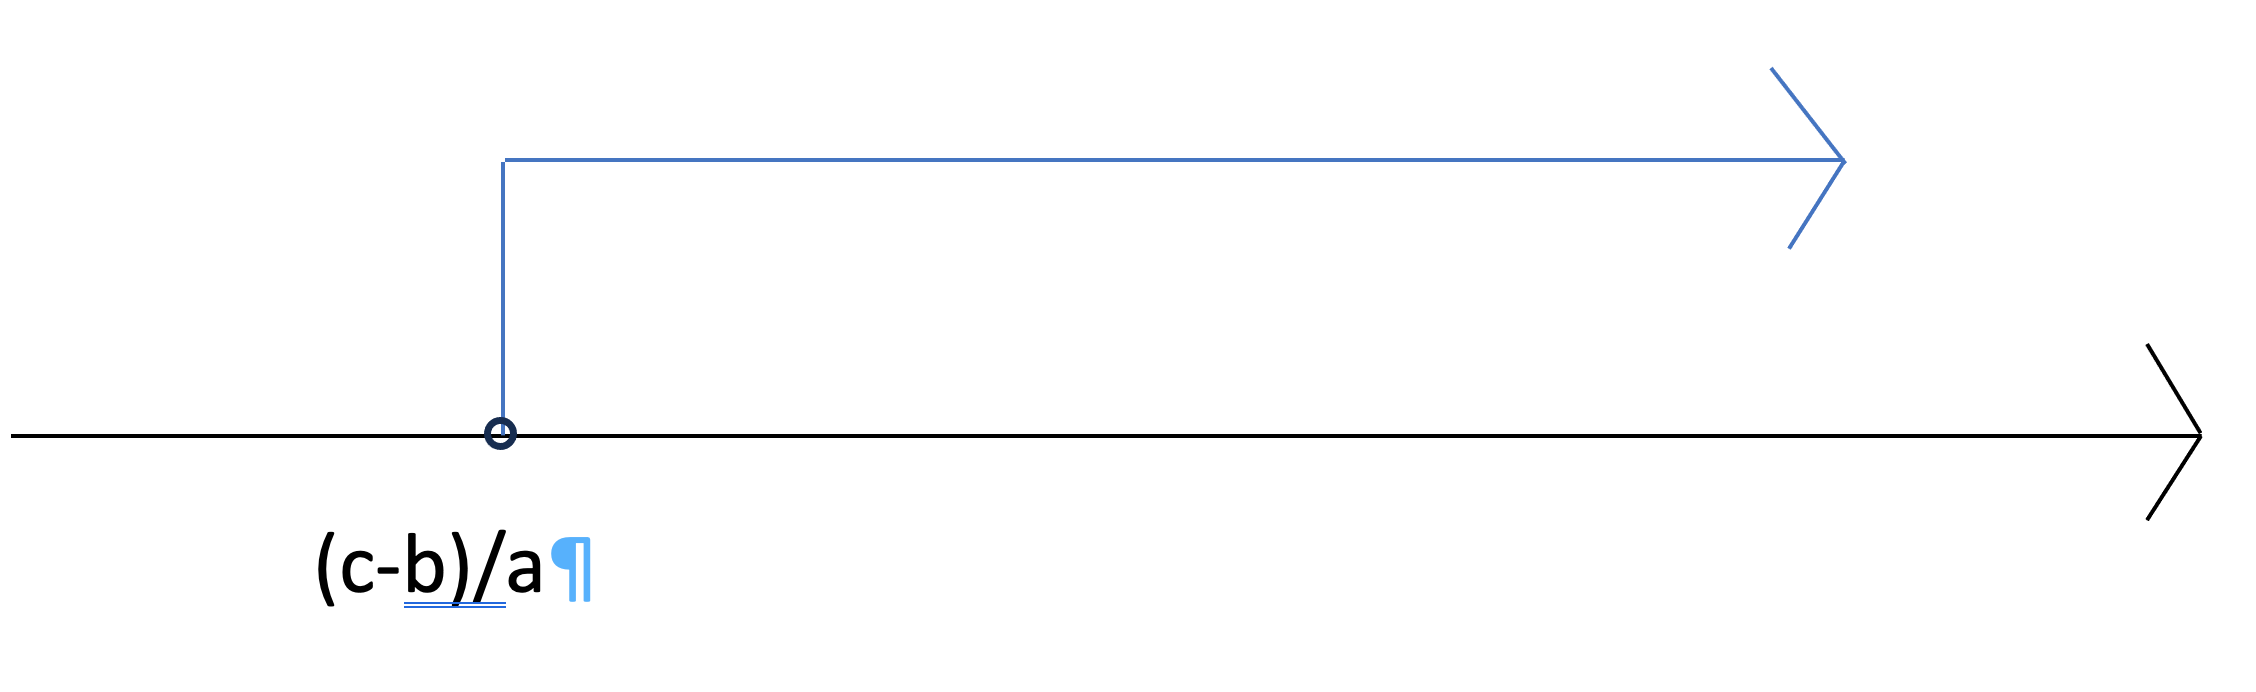
\includegraphics[width=3.12500in]{Desigualdad1.png}
\caption{Desigualdad \(ax+b>c\)}
\end{figure}

\begin{Ejem}
Supongamos se tiene la desigualdad $ax+b\leq c$, con $a\neq0$: 

\begin{eqnarray*}
ax+b&\leq&c\\
ax+b-b&\leq&c-b\\
ax&\leq&c-b\\
\left(\frac{1}{a}\right)ax&\leq&\left(\frac{1}{a}\right)\left(c-b\right)\\
\left(\frac{1}{a}\times a\right)x&\leq&\frac{c-b}{a}\\
\left(\frac{a}{a}\right)x&\leq&\frac{c-b}{a}\\
\left(1\right)x&\leq&\frac{c-b}{a}\\
x&\leq&\frac{c-b}{a}
\end{eqnarray*}
\begin{flushright}
$\blacksquare$
\end{flushright}

\end{Ejem}

\begin{figure}
\centering
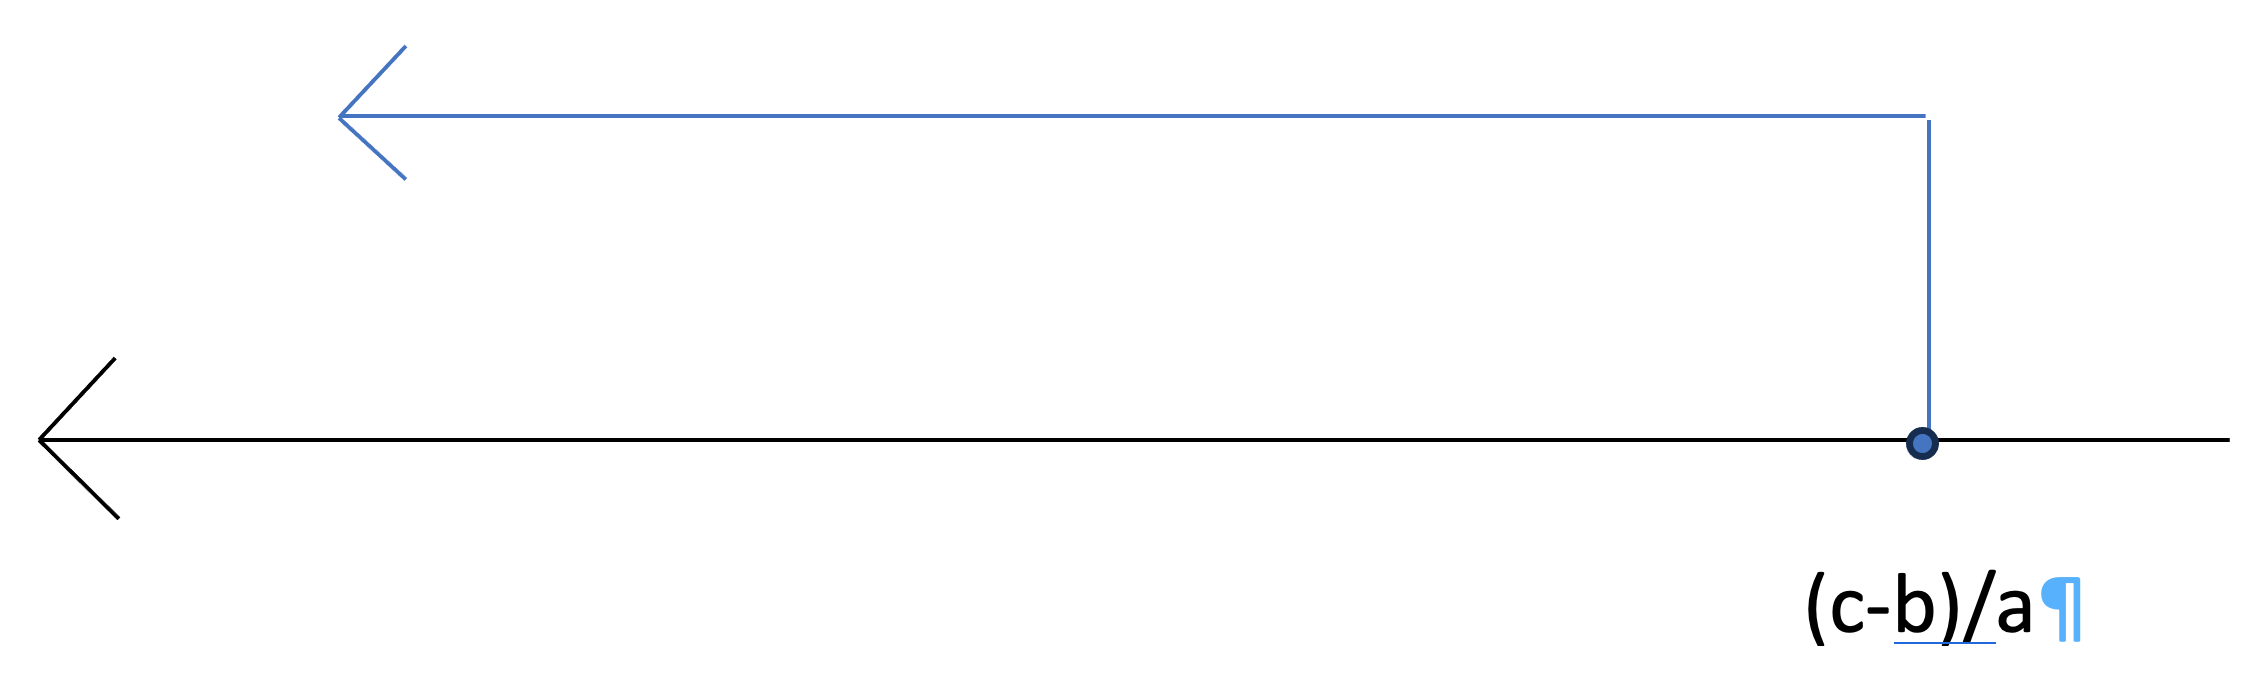
\includegraphics[width=3.12500in]{Desigualdad2.png}
\caption{Desigualdad \(ax+b\leq c\)}
\end{figure}

\begin{Ejem}
Supongamos se tiene la desigualdad $c\leq ax+b\leq d$, con $a\neq0$: 

\begin{eqnarray*}
c&\leq& ax+b<d\\
c-b&\leq& ax+b-b<d-b\\
c-b&\leq& ax+0<d-b\\
c-b&\leq& ax<d-b\\
\left(\frac{1}{a}\right)c-b&\leq& \left(\frac{1}{a}\right)ax<\left(\frac{1}{a}\right)d-b\\
\left(\frac{c-b}{a}\right)&\leq& \left(\frac{a}{a}\right)x<\left(\frac{d-b}{a}\right)\\
\left(\frac{c-b}{a}\right)&\leq& x<\left(\frac{d-b}{a}\right)\\
\end{eqnarray*}
\begin{flushright}
$\blacksquare$
\end{flushright}

\end{Ejem}

\begin{figure}
\centering
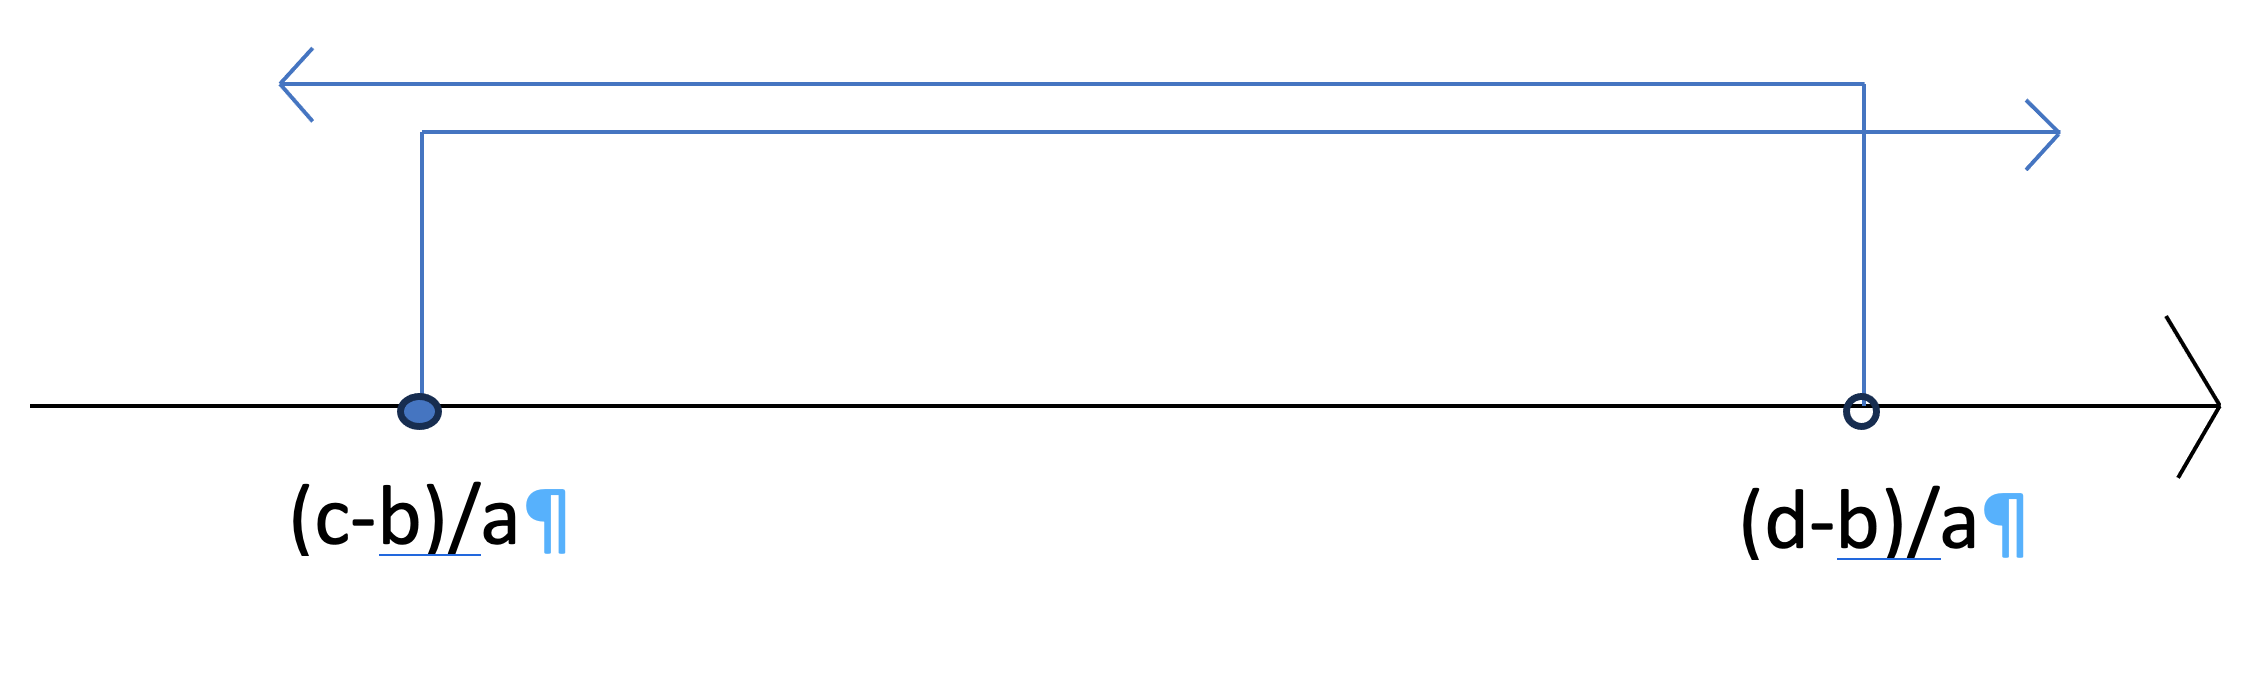
\includegraphics[width=3.12500in]{Desigualdad3.png}
\caption{Desigualdad \(c\leq ax+b\leq d\), con \(a\neq0\)}
\end{figure}

\begin{Ejem}
Supongamos se tiene la desigualdad $|ax+b|\leq c$, con $a\neq0$, recordemos que $|a|=b$, sí y sólo si $a=b$ o $a=-b$, entonces

\begin{eqnarray*}
|ax+b|&\leq& c\\
-c&\leq& ax+b \leq c\\
-c-b&\leq& ax+b-b \leq c-b\\
-c-b&\leq& ax+0<c-b\\
-c-b&\leq& ax<c-b\\
\left(\frac{1}{a}\right)c-b&\leq& \left(\frac{1}{a}\right)ax<\left(\frac{1}{a}\right)c-b\\
\left(\frac{-c-b}{a}\right)&\leq& \left(\frac{a}{a}\right)x<\left(\frac{c-b}{a}\right)\\
\left(\frac{-c-b}{a}\right)&\leq& x<\left(\frac{c-b}{a}\right)\\
-\left(\frac{c+b}{a}\right)&\leq& x<\left(\frac{c-b}{a}\right)\\
\end{eqnarray*}
\begin{flushright}
$\blacksquare$
\end{flushright}

\end{Ejem}

\begin{figure}
\centering
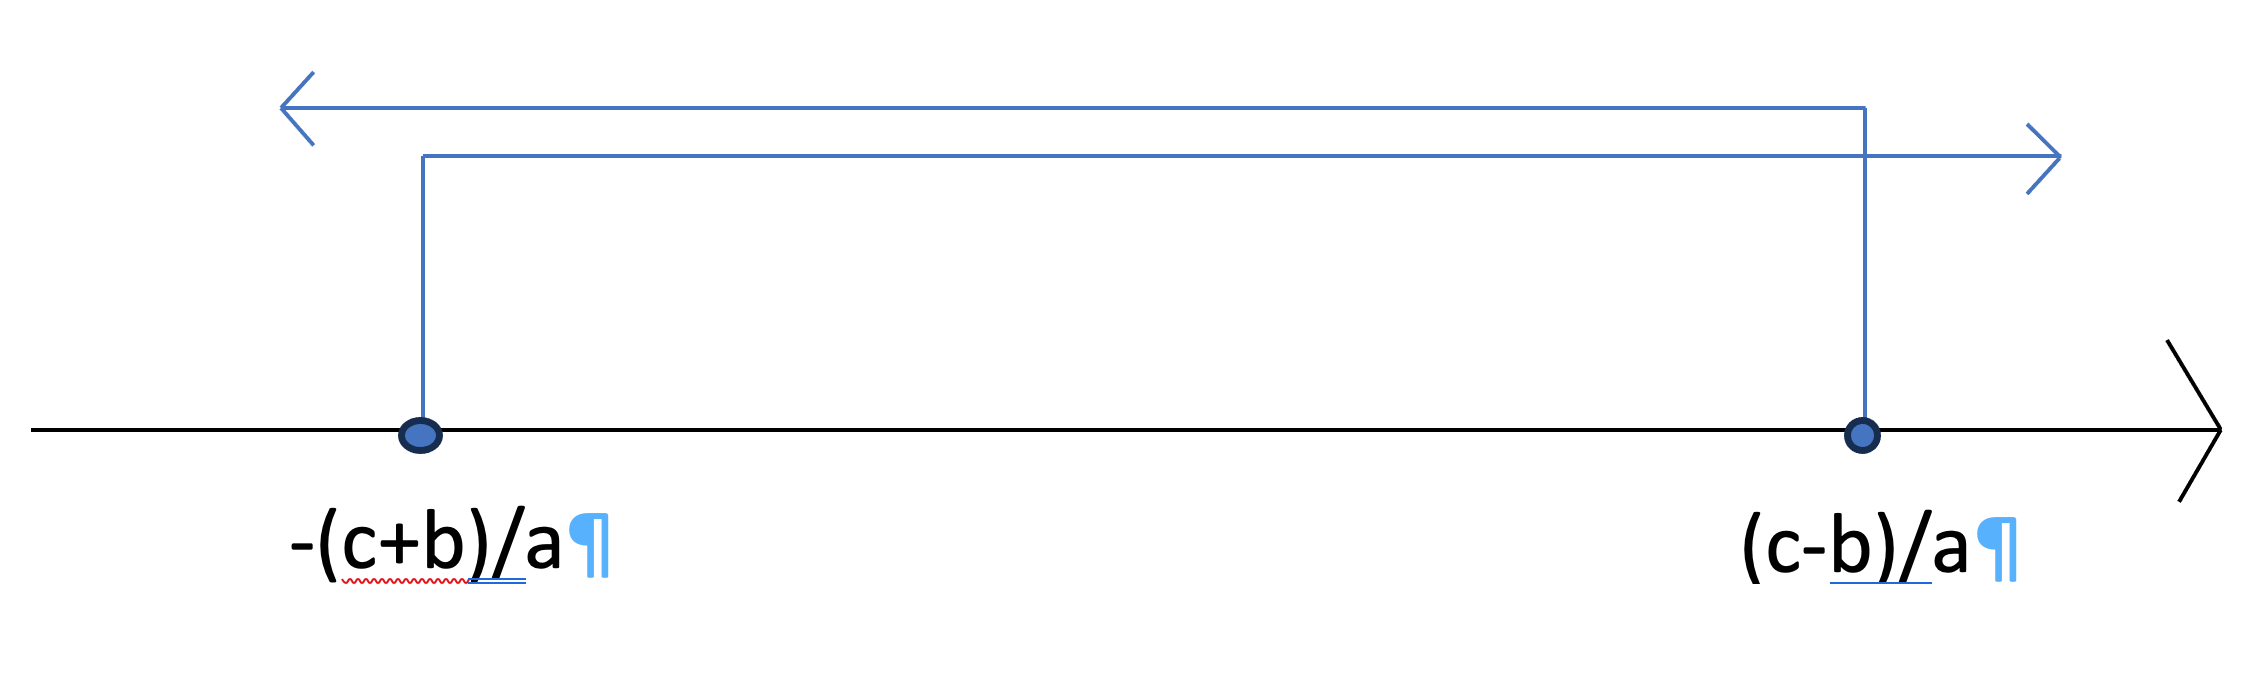
\includegraphics[width=3.12500in]{Desigualdad4.png}
\caption{Desigualdad \(|ax+b|\leq c\), con \(a\neq0\)}
\end{figure}

\begin{Ejem}
Supongamos se tiene la desigualdad $|ax+b|\geq c$, con $a\neq0$, recordemos que $|a|\geq b$ sí y sólo sí, $a\geq b$ o $a\leq -b$, entonces tenemos dos casos

\begin{itemize}
\item[Caso 1:]
\begin{eqnarray*}
ax+b&\geq& c\\
ax+b-b&\geq& c-b\\
ax+0&\geq& c-b\\
ax&\geq& c-b\\
\left(\frac{1}{a}\right)ax&\geq&\left(\frac{1}{a}\right)c-b\\
\left(\frac{a}{a}\right)ax&\geq&\left(\frac{1}{a}\right)c-b\\
\left(1\right)x&\geq&\left(\frac{c-b}{a}\right)\\
x&\geq&\left(\frac{c-b}{a}\right)
\end{eqnarray*}


\item[Caso 2:]
\begin{eqnarray*}
ax+b&\leq& -c\\
ax+b-b&\leq& -c-b\\
ax+0&\leq& -c-b\\
ax&\leq& -c-b\\
\left(\frac{1}{a}\right)ax&\leq&\left(\frac{1}{a}\right)\left(-c-b\right)\\
\left(\frac{a}{a}\right)ax&\leq&\left(\frac{1}{a}\right)\left(-c-b\right)\\
\left(1\right)x&\leq&-\left(\frac{c+b}{a}\right)\\
x&\leq&-\left(\frac{c+b}{a}\right)\\
\end{eqnarray*}

\end{itemize}

\begin{flushright}
$\blacksquare$
\end{flushright}

\end{Ejem}

\begin{figure}
\centering
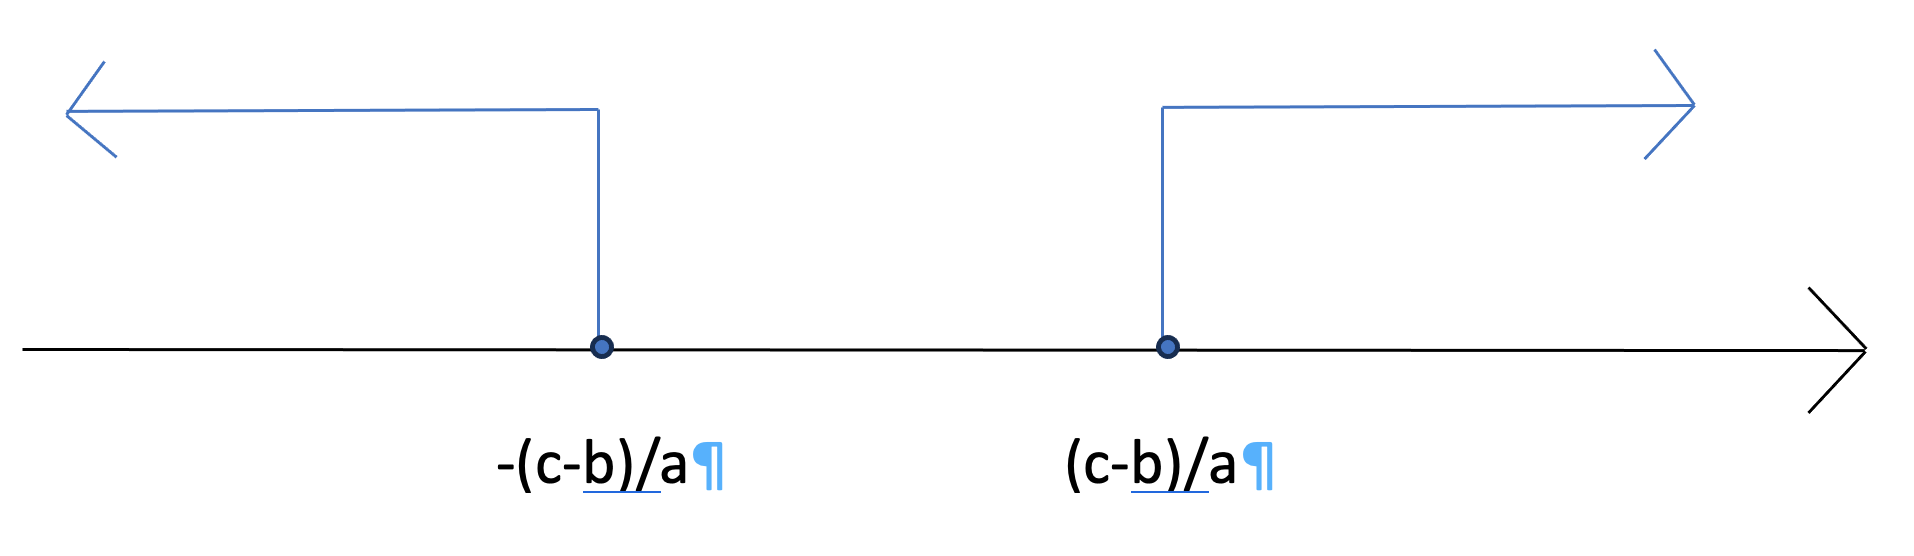
\includegraphics[width=3.12500in]{Desigualdad5.png}
\caption{Desigualdad \(|ax+b|\leq c\), con \(a\neq0\)}
\end{figure}

\section{Solución de desigualdades de primer
grado}\label{soluciuxf3n-de-desigualdades-de-primer-grado}

\subsection{\texorpdfstring{Solución de desigualdades del tipo:
\(ax+b>c\)}{Solución de desigualdades del tipo: ax+b\textgreater{}c}}\label{soluciuxf3n-de-desigualdades-del-tipo-axbc}

\textbf{Resuelve las siguientes desigualdades, proporcionando el
conjunto solución, el intervalo solución así como la representación
gráfica de la misma}

\begin{multicols}{3}
1. $2x+3>7$

2. $-5x+2>9$

3. $4x-1>3$

4. $-3x+5>8$

5. $2x+1>3x-2$

6. $3x-2>2x+4$

7. $4x+1>2x+5$

8. $-2x-3>4x-7$

9. $5x-2>3x+4$

10. $2x+4>6x-8$

11. $-4x+3>5x-2$

12. $3x-1>4x-3$

13. $2x-5>x-3$

14. $3x+2>2x-5$

15. $-2x+1>5x-8$
\end{multicols}

\subsection{\texorpdfstring{Solución de desigualdades del tipo:
\(ax+b>c\), con coeficientes
fraccionarios}{Solución de desigualdades del tipo: ax+b\textgreater{}c, con coeficientes fraccionarios}}\label{soluciuxf3n-de-desigualdades-del-tipo-axbc-con-coeficientes-fraccionarios}

\textbf{Resuelve las siguientes desigualdades, proporcionando el
conjunto solución, el intervalo solución así como la representación
gráfica de la misma}

\begin{multicols}{3}
1. $\frac{1}{2}x+\frac{3}{4}>1$

2. $-\frac{2}{3}x+\frac{4}{5}>3$

3. $\frac{3}{4}x-\frac{1}{2}>\frac{5}{6}$

4. $-\frac{2}{5}x+\frac{1}{3}>-\frac{1}{15}$

5. $\frac{2}{3}x+\frac{1}{4}>\frac{5}{6}x-\frac{1}{2}$

6. $\frac{1}{2}x-\frac{1}{3}>-\frac{2}{5}x+\frac{7}{15}$

7. $-\frac{3}{4}x+\frac{1}{2}>\frac{2}{3}x-\frac{1}{4}$

8. $\frac{1}{3}x-\frac{2}{5}>\frac{2}{7}x-\frac{1}{7}$

9. $\frac{2}{5}x+\frac{1}{6}\geq\frac{1}{3}x+\frac{5}{6}$

10. $\frac{3}{4}x+\frac{1}{5}>\frac{1}{2}x+\frac{3}{10}$

11. $-\frac{1}{2}x+\frac{1}{3}>-\frac{3}{4}x-\frac{1}{6}$

12. $\frac{1}{4}x-\frac{1}{2}>\frac{2}{3}x-\frac{4}{6}$

13. $\frac{2}{3}x-\frac{1}{4}>\frac{3}{4}x-\frac{2}{3}$

14. $-\frac{1}{2}x+\frac{3}{4}>\frac{3}{5}x+\frac{1}{10}$

15. $\frac{2}{5}x-\frac{1}{4}>-\frac{1}{2}x+\frac{3}{8}$
\end{multicols}

\subsection{\texorpdfstring{Solución de desigualdades del tipo:
\(ax+b<c\)}{Solución de desigualdades del tipo: ax+b\textless{}c}}\label{soluciuxf3n-de-desigualdades-del-tipo-axbc-1}

\textbf{Resuelve las siguientes desigualdades, proporcionando el
conjunto solución, el intervalo solución así como la representación
gráfica de la misma}

\begin{multicols}{3}
1. $2x+3<7$

2. $-5x+2<-9$

3. $4x-1<3$

4. $-3x+5<8$

5. $2x+1<3x-2$

6. $3x-2<2x+4$

7. $4x+1<2x+5$

8. $-2x-3<4x-7$

9. $5x-2<3x+4$

10. $2x+4<6x-8$

11. $-4x+3<5x-2$

12. $3x-1<4x-3$

13. $2x-5<x-3$

14. $3x+2<2x-5$

15. $-2x+1<5x-8$
\end{multicols}

\subsection{\texorpdfstring{Solución de desigualdades del tipo:
\(ax+b<c\) con coeficientes
fraccionarios}{Solución de desigualdades del tipo: ax+b\textless{}c con coeficientes fraccionarios}}\label{soluciuxf3n-de-desigualdades-del-tipo-axbc-con-coeficientes-fraccionarios-1}

\textbf{Resuelve las siguientes desigualdades, proporcionando el
conjunto solución, el intervalo solución así como la representación
gráfica de la misma}

\begin{multicols}{3}
1. $\frac{1}{2}x+\frac{3}{4}<\frac{5}{8}$

2. $-\frac{2}{3}x+\frac{4}{5}<\frac{1}{2}$

3. $\frac{3}{4}x-\frac{1}{2}<\frac{5}{6}$

4. $-\frac{2}{5}x+\frac{1}{3}<-\frac{1}{15}$

5. $\frac{2}{3}x+\frac{1}{4}<\frac{5}{6}x-\frac{1}{2}$

6. $\frac{1}{2}x-\frac{1}{3}<\frac{2}{5}x-\frac{7}{15}$

7. $-\frac{3}{4}x+\frac{1}{2}<\frac{2}{3}x-\frac{1}{4}$

8. $\frac{1}{3}x-\frac{2}{5}<\frac{2}{7}x-\frac{1}{7}$

9. $\frac{2}{5}x+\frac{1}{6}<\frac{1}{3}x+\frac{5}{6}$

10. $\frac{3}{4}x+\frac{1}{5}<\frac{1}{2}x+\frac{3}{10}$

11. $-\frac{1}{2}x+\frac{1}{3}<-\frac{3}{4}x-\frac{1}{6}$

12. $\frac{1}{4}x-\frac{1}{2}<\frac{2}{3}x-\frac{4}{6}$

13. $\frac{2}{3}x-\frac{1}{4}<\frac{3}{4}x-\frac{2}{3}$

14. $-\frac{1}{2}x+\frac{3}{4}<\frac{3}{5}x+\frac{1}{10}$

15. $\frac{2}{5}x-\frac{1}{4}<-\frac{1}{2}x+\frac{3}{8}$
\end{multicols}

\subsection{\texorpdfstring{Solución de desigualdades del tipo:
\(ax+b \geq c\)}{Solución de desigualdades del tipo: ax+b \textbackslash{}geq c}}\label{soluciuxf3n-de-desigualdades-del-tipo-axb-geq-c}

\textbf{Resuelve las siguientes desigualdades, proporcionando el
conjunto solución, el intervalo solución así como la representación
gráfica de la misma}

\begin{multicols}{3}
1. $2x + 3 \geq 5$

2. $-4x + 2 \geq -10$

3. $5x - 4 \geq 6$

4. $-3x + 7 \geq 4$

5. $2x - 3 \geq x + 2$

6. $3x + 2 \geq 2x - 1$

7. $4x - 1 \geq x + 5$

8. $-2x - 3 \geq -6x - 1$

9. $5x - 2 \geq 2x + 8$

10. $2x + 4 \geq 4x - 2$

11. $-4x + 3 \geq 3x - 2$

12. $3x - 1 \geq 2x + 1$

13. $2x - 5 \geq x - 1$

14. $3x + 2 \geq 2x - 4$

15. $-2x + 1 \geq -5x + 4$
\end{multicols}

\subsection{\texorpdfstring{Solución de desigualdades del tipo:
\(ax+b \geq c\), con coeficientes
fraccionarios}{Solución de desigualdades del tipo: ax+b \textbackslash{}geq c, con coeficientes fraccionarios}}\label{soluciuxf3n-de-desigualdades-del-tipo-axb-geq-c-con-coeficientes-fraccionarios}

\textbf{Resuelve las siguientes desigualdades, proporcionando el
conjunto solución, el intervalo solución así como la representación
gráfica de la misma}

\begin{multicols}{3}
1. $\frac{1}{2}x + \frac{3}{4} \geq \frac{5}{8}$

2. $-\frac{2}{3}x + \frac{4}{5} \geq \frac{1}{2}$

3. $\frac{3}{4}x - \frac{1}{2} \geq \frac{5}{6}$

4. $-\frac{2}{5}x + \frac{1}{3} \geq -\frac{1}{15}$

5. $\frac{2}{3}x + \frac{1}{4} \geq \frac{5}{6}x - \frac{1}{2}$

6. $\frac{1}{2}x - \frac{1}{3} \geq \frac{2}{5}x - \frac{7}{15}$

7. $-\frac{3}{4}x + \frac{1}{2} \geq \frac{2}{3}x - \frac{1}{4}$

8. $\frac{1}{3}x - \frac{2}{5} \geq \frac{2}{7}x - \frac{1}{7}$

9. $\frac{2}{5}x + \frac{1}{6} \geq \frac{1}{3}x + \frac{5}{6}$

10. $\frac{3}{4}x + \frac{1}{5} \geq \frac{1}{2}x + \frac{3}{10}$

11. $-\frac{1}{2}x + \frac{1}{3} \geq -\frac{3}{4}x - \frac{1}{6}$

12. $\frac{1}{4}x - \frac{1}{2} \geq \frac{2}{3}x - \frac{4}{6}$

13. $\frac{2}{3}x - \frac{1}{4} \geq \frac{3}{4}x - \frac{2}{3}$

14. $-\frac{1}{2}x + \frac{3}{4} \geq \frac{3}{5}x + \frac{1}{10}$

15. $\frac{2}{5}x - \frac{1}{4} \geq -\frac{1}{2}x + \frac{3}{8}$
\end{multicols}

\subsection{\texorpdfstring{Solución de desigualdades del tipo:
\(ax+b \leq c\)}{Solución de desigualdades del tipo: ax+b \textbackslash{}leq c}}\label{soluciuxf3n-de-desigualdades-del-tipo-axb-leq-c}

\textbf{Resuelve las siguientes desigualdades, proporcionando el
conjunto solución, el intervalo solución así como la representación
gráfica de la misma}

\begin{multicols}{3}
1. $2x + 3 \leq 7$

2. $-3x + 4 \leq 5$

3. $4x - 2 \leq 6$

4. $-5x + 3 \leq 2$

5. $2x + 1 \leq 5x - 2$

6. $3x - 1 \leq 5x + 2$

7. $-4x + 2 \leq 3x + 1$

8. $3x - 5 \leq 7x - 2$

9. $5x + 1 \leq 3x + 4$

10. $4x + 1 \leq 6x - 3$

11. $-2x + 3 \leq -4x - 1$

12. $x - 2 \leq 2x + 1$

13. $3x - 4 \leq 4x - 2$

14. $-2x + 4 \leq 5x + 1$

15. $2x - 1 \leq -3x + 4$
\end{multicols}

\subsection{\texorpdfstring{Solución de desigualdades del tipo:
\(ax+b \leq c\) con coeficientes
fraccionarios.}{Solución de desigualdades del tipo: ax+b \textbackslash{}leq c con coeficientes fraccionarios.}}\label{soluciuxf3n-de-desigualdades-del-tipo-axb-leq-c-con-coeficientes-fraccionarios.}

\textbf{Resuelve las siguientes desigualdades, proporcionando el
conjunto solución, el intervalo solución así como la representación
gráfica de la misma}

\begin{multicols}{3}
1. $\frac{1}{2}x + \frac{3}{4} \leq \frac{5}{8}$

2. $-\frac{2}{3}x + \frac{4}{5} \leq \frac{1}{2}$

3. $\frac{3}{4}x - \frac{1}{2} \leq \frac{5}{6}$

4. $-\frac{2}{5}x + \frac{1}{3} \leq -\frac{1}{15}$

5. $\frac{2}{3}x + \frac{1}{4} \leq \frac{5}{6}x - \frac{1}{2}$

6. $\frac{1}{2}x - \frac{1}{3} \leq \frac{2}{5}x - \frac{7}{15}$

7. $-\frac{3}{4}x + \frac{1}{2} \leq \frac{2}{3}x - \frac{1}{4}$

8. $\frac{1}{3}x - \frac{2}{5} \leq \frac{2}{7}x - \frac{1}{7}$

9. $\frac{2}{5}x + \frac{1}{6} \leq \frac{1}{3}x + \frac{5}{6}$

10. $\frac{3}{4}x + \frac{1}{5} \leq \frac{1}{2}x + \frac{3}{10}$

11. $-\frac{1}{2}x + \frac{1}{3} \leq -\frac{3}{4}x - \frac{1}{6}$

12. $\frac{1}{4}x - \frac{1}{2} \leq \frac{2}{3}x - \frac{4}{6}$

13. $\frac{2}{3}x - \frac{1}{4} \leq \frac{3}{4}x - \frac{2}{3}$

14. $-\frac{1}{2}x + \frac{3}{4} \leq \frac{3}{5}x + \frac{1}{10}$

15. $\frac{2}{5}x - \frac{1}{4} \leq -\frac{1}{2}x + \frac{3}{8}$
\end{multicols}

\section{Solución de desigualdades con doble
desigualdad.}\label{soluciuxf3n-de-desigualdades-con-doble-desigualdad.}

\subsection{\texorpdfstring{Solución de desigualdades del tipo:
\(c< ax+b <d\)}{Solución de desigualdades del tipo: c\textless{} ax+b \textless{}d}}\label{soluciuxf3n-de-desigualdades-del-tipo-c-axb-d}

\textbf{Resuelve las siguientes desigualdades, proporcionando el
conjunto solución, el intervalo solución así como la representación
gráfica de la misma}

\begin{multicols}{3}
1. $2<x+3<5$

2. $-1<2x-1<1$

3. $-\frac{1}{2}<\frac{3}{4}x+\frac{1}{2}<\frac{1}{2}$

4. $-3< 2x+7<-1$

5. $1<\frac{1}{2}x-\frac{1}{4}<2$

6. $-5<-\frac{1}{3}x+\frac{5}{6}<1$

7. $-5<5x-1<8$

8. $-2< \frac{2}{3}x+1<12$

9. $2<-\frac{1}{2}x+\frac{3}{4}<3$

10. $-3< \frac{1}{2}x-\frac{1}{3}<18$

11. $-4< -3x+5<3$

12. $1<\frac{1}{2}x+\frac{1}{3}<2$

13. $-2< 4x-1<2$

14. $-\frac{3}{4}<\frac{1}{2}x-\frac{1}{4}<\frac{3}{4}$

15. $-1<s\frac{3}{2}x+1<2$
\end{multicols}

\subsection{\texorpdfstring{Solución de desigualdades del tipo:
\(c< ax+b \leq d\)}{Solución de desigualdades del tipo: c\textless{} ax+b \textbackslash{}leq d}}\label{soluciuxf3n-de-desigualdades-del-tipo-c-axb-leq-d}

\textbf{Resuelve las siguientes desigualdades, proporcionando el
conjunto solución, el intervalo solución así como la representación
gráfica de la misma}

\begin{multicols}{3}
1. $-2<3x+1\leq 5$

2. $-\frac{4}{5}< \frac{1}{2}x-\frac{3}{4}\leq2$

3. $-1<2x-1\leq 1$

4. $-3< \frac{1}{2}x+\frac{1}{3}\leq \frac{8}{5}$

5. $-\frac{3}{4}<\frac{1}{2}x+\frac{1}{4}\leq \frac{3}{4}$

6. $-2<\frac{3}{2}x-1\leq 1$

7. $-1<\frac{2}{3}x+1\leq \frac{8}{3}$

8. $1<\frac{1}{2}x+\frac{1}{3}\leq 2$

9. $-3< -2x+5\leq 3$

10. $-\frac{1}{2}<\frac{3}{4}x+\frac{1}{2}\leq \frac{1}{2}$

11. $-5<5x-1\leq 9$

12. $1<\frac{1}{2}x-\frac{1}{4}\leq 2$

13. $-3< 2x+7\leq -1$

14. $-1< -\frac{1}{2}x+\frac{1}{4}\leq 2$

15. $2<-\frac{1}{2}x+\frac{3}{4}\leq 3$
\end{multicols}

\subsection{\texorpdfstring{Solución de desigualdades del tipo:
\(c\leq ax+b <d\)}{Solución de desigualdades del tipo: c\textbackslash{}leq ax+b \textless{}d}}\label{soluciuxf3n-de-desigualdades-del-tipo-cleq-axb-d}

\textbf{Resuelve las siguientes desigualdades, proporcionando el
conjunto solución, el intervalo solución así como la representación
gráfica de la misma}

\begin{multicols}{3}
1. $-2\leq 3x+1<5$

2. $-\frac{4}{5}\leq \frac{1}{2}x-\frac{3}{4}<2$

3. $-1\leq 2x-1<1$

4. $-3\leq \frac{1}{2}x+\frac{1}{3}<\frac{7}{9}$

5. $-\frac{3}{4}\leq \frac{1}{2}x+\frac{1}{4}<\frac{3}{4}$

6. $-2\leq \frac{3}{2}x-1<1$

7. $-1\leq \frac{2}{3}x+1<\frac{9}{4}$

8. $1\leq \frac{1}{2}x+\frac{1}{3}<2$

9. $-\frac{4}{3}\leq -2x+5<3$

10. $-\frac{1}{2}\leq \frac{3}{4}x+\frac{1}{2}<\frac{1}{2}$

11. $-5\leq 5x-1<\frac{15}{6}$

12. $1\leq \frac{1}{2}x-\frac{1}{4}<2$

13. $-3\leq 2x+7<-1$

14. $-1\leq -\frac{1}{2}x+\frac{1}{4}<2$

15. $2\leq -\frac{1}{2}x+\frac{3}{4}<3$
\end{multicols}

\subsection{\texorpdfstring{Solución de desigualdades del tipo:
\(c\leq ax+b \leq d\)}{Solución de desigualdades del tipo: c\textbackslash{}leq ax+b \textbackslash{}leq d}}\label{soluciuxf3n-de-desigualdades-del-tipo-cleq-axb-leq-d}

\textbf{Resuelve las siguientes desigualdades, proporcionando el
conjunto solución, el intervalo solución así como la representación
gráfica de la misma}

\begin{multicols}{3}
1. $-1\leq x\leq 2$

2. $-\frac{3}{4}\leq \frac{1}{2}x+\frac{1}{4}\leq \frac{5}{8}$

3. $2\leq 3x-1\leq 7$

4. $-\frac{1}{3}\leq \frac{1}{6}x+\frac{1}{2}\leq \frac{1}{2}$

5. $-1\leq -x+3\leq 2$

6. $-2\leq \frac{1}{2}x+1\leq 3$

7. $2\leq \frac{3}{2}x+1\leq 5$

8. $-\frac{3}{4}\leq -\frac{1}{2}x+\frac{1}{4}\leq \frac{1}{4}$

9. $-4\leq 2x+1\leq 7$

10. $-\frac{1}{2}\leq -\frac{3}{4}x+\frac{1}{2}\leq 1$

11. $-\frac{5}{2}\leq \frac{1}{4}x+1\leq 1$

12. $1\leq -\frac{1}{2}x+\frac{3}{4}\leq 3$

13. $-\frac{5}{6}\leq \frac{1}{3}x+\frac{1}{2}\leq \frac{1}{2}$

14. $-1\leq \frac{1}{2}x-\frac{1}{4}\leq 3$

15. $-2\leq \frac{1}{4}x+\frac{1}{2}\leq 3$
\end{multicols}

\section{Solución de desigualdades con valor
absoluto}\label{soluciuxf3n-de-desigualdades-con-valor-absoluto}

\subsection{\texorpdfstring{Solución de desigualdades del tipo:
\(|ax+b| <d\)}{Solución de desigualdades del tipo: \textbar{}ax+b\textbar{} \textless{}d}}\label{soluciuxf3n-de-desigualdades-del-tipo-axb-d}

\textbf{Resuelve las siguientes desigualdades, proporcionando el
conjunto solución, el intervalo solución así como la representación
gráfica de la misma}

\begin{multicols}{3}
1. $|2x+1|<5$

2. $|\frac{1}{2}x-\frac{1}{4}|<2$

3. $|3x-1|<7$

4. $|\frac{1}{3}x+\frac{1}{2}|<1$

5. $|x-2|<4$

6. $|\frac{1}{2}x+1|<3$

7. $|\frac{3}{2}x+1|<5$

8. $|\frac{1}{2}x-\frac{1}{4}|<\frac{3}{4}$

9. $|2x+1|<6$

10. $|\frac{3}{4}x-\frac{1}{2}|<1$

11. $|\frac{1}{4}x+1|<\frac{7}{2}$

12. $|-\frac{1}{2}x+\frac{3}{4}|<2$

13. $|\frac{1}{3}x+\frac{1}{2}|<\frac{5}{6}$

14. $|\frac{1}{2}x-\frac{1}{4}|<3$

15. $|\frac{1}{4}x+\frac{1}{2}|<\frac{7}{4}$
\end{multicols}

\subsection{\texorpdfstring{Solución de desigualdades del tipo:
\(|ax+b| \leq d\)}{Solución de desigualdades del tipo: \textbar{}ax+b\textbar{} \textbackslash{}leq d}}\label{soluciuxf3n-de-desigualdades-del-tipo-axb-leq-d}

\textbf{Resuelve las siguientes desigualdades, proporcionando el
conjunto solución, el intervalo solución así como la representación
gráfica de la misma}

\begin{multicols}{3}
1. $|3x-1|\leq 6$

2. $|\frac{1}{2}x-\frac{1}{4}|\leq 1$

3. $|2x+1|\leq 5$

4. $|\frac{1}{3}x+\frac{1}{2}|\leq \frac{4}{3}$

5. $|x-2|\leq 3$

6. $|\frac{1}{2}x+1|\leq 4$

7. $|\frac{3}{2}x+1|\leq 5$

8. $|\frac{1}{2}x-\frac{1}{4}|\leq \frac{5}{4}$

9. $|2x+1|\leq 7$

10. $|\frac{3}{4}x-\frac{1}{2}|\leq 2$

11. $|\frac{1}{4}x+1|\leq 3$

12. $|-\frac{1}{2}x+\frac{3}{4}|\leq 2$

13. $|\frac{1}{3}x+\frac{1}{2}|\leq 1$

14, $|\frac{1}{2}x-\frac{1}{4}|\leq 2$

15. $|\frac{1}{4}x+\frac{1}{2}|\leq \frac{5}{4}$
\end{multicols}

\subsection{\texorpdfstring{Solución de desigualdades del tipo:
\(|ax+b| >d\)}{Solución de desigualdades del tipo: \textbar{}ax+b\textbar{} \textgreater{}d}}\label{soluciuxf3n-de-desigualdades-del-tipo-axb-d-1}

\textbf{Resuelve las siguientes desigualdades, proporcionando el
conjunto solución, el intervalo solución así como la representación
gráfica de la misma}

\begin{multicols}{3}
1. $|3x-1|>4$

2. $|\frac{1}{2}x-\frac{1}{4}|>\frac{1}{2}$

3. $|2x+1|>3$

4. $|\frac{1}{3}x+\frac{1}{2}|>\frac{5}{6}$

5. $|x-2|>1$

6. $|\frac{1}{2}x+1|>\frac{3}{4}$

7. $|\frac{3}{2}x+1|>\frac{7}{2}$

8. $|\frac{1}{2}x-\frac{1}{4}|>\frac{3}{4}$

9. $|2x+1|>\frac{9}{2}$

10. $|\frac{3}{4}x-\frac{1}{2}|>\frac{5}{4}$

11. $|\frac{1}{4}x+1|>1$

12. $|-\frac{1}{2}x+\frac{3}{4}|>\frac{1}{2}$

13. $|\frac{1}{3}x+\frac{1}{2}|>\frac{2}{3}$

14. $|\frac{1}{2}x-\frac{1}{4}|>\frac{5}{4}$

15. $|\frac{1}{4}x+\frac{1}{2}|>1$
\end{multicols}

\subsection{\texorpdfstring{Solución de desigualdades del tipo:
\(|ax+b| \geq d\)}{Solución de desigualdades del tipo: \textbar{}ax+b\textbar{} \textbackslash{}geq d}}\label{soluciuxf3n-de-desigualdades-del-tipo-axb-geq-d}

\textbf{Resuelve las siguientes desigualdades, proporcionando el
conjunto solución, el intervalo solución así como la representación
gráfica de la misma}

\begin{multicols}{3}
1. $|3x-1|\geq 4$

2. $|\frac{1}{2}x-\frac{1}{4}|\geq\frac{1}{2}$

3. $|2x+1|\geq 3$

4. $|\frac{1}{3}x+\frac{1}{2}|\geq\frac{5}{6}$

5. $|x-2|\geq 1$

6. $|\frac{1}{2}x+1|\geq\frac{3}{4}$

7. $|\frac{3}{2}x+1|\geq\frac{7}{2}$

8. $|\frac{1}{2}x-\frac{1}{4}|\geq\frac{3}{4}$

9. $|2x+1|\geq\frac{9}{2}$

10. $|\frac{3}{4}x-\frac{1}{2}|\geq\frac{5}{4}$

11. $|\frac{1}{4}x+1|\geq 1$

12. $|-\frac{1}{2}x+\frac{3}{4}|\geq\frac{1}{2}$

13. $|\frac{1}{3}x+\frac{1}{2}|\geq\frac{2}{3}$

14. $|\frac{1}{2}x-\frac{1}{4}|\geq\frac{5}{4}$

15. $|\frac{1}{4}x+\frac{1}{2}|\geq 1$
\end{multicols}

\subsection{Ejercicios adicionales}\label{ejercicios-adicionales}

\begin{enumerate}
\def\labelenumi{\arabic{enumi}.}
\tightlist
\item
  Resuelve los ejercicios siguientes, encuentra el intervalo solución y
  proporciona su gráfica
\end{enumerate}

\begin{multicols}{2}
    i. $|-\frac{1}{3}x+\frac{2}{5}| \leq \frac{4}{5}$
    
    ii. $|-\frac{2}{7}x-\frac{3}{4}| \leq \frac{2}{3}$
    
    iii. $|\frac{5}{8}x-\frac{1}{6}| \leq \frac{7}{8}$
    
    iv. $|\frac{3}{10}x+\frac{2}{9}| \leq \frac{1}{2}$
    
    v. $|-\frac{4}{11}x+\frac{5}{7}| \leq \frac{3}{4}$
    
    vi. $|-\frac{2}{5}x-\frac{1}{3}| \leq \frac{2}{5}$
    
    vii. $|\frac{1}{6}x+\frac{7}{9}| \leq \frac{1}{3}$
    
    viii. $|\frac{7}{9}x-\frac{4}{11}| \leq \frac{5}{6}$
    
    ix. $|-\frac{5}{8}x+\frac{3}{10}| \leq \frac{2}{7}$
    
    x. $|-\frac{1}{4}x-\frac{1}{8}| \leq \frac{3}{4}$
    
    xi. $|\frac{3}{7}x+\frac{5}{6}| \leq \frac{1}{5}$
    
    xii. $|-\frac{4}{9}x+\frac{2}{11}| \leq \frac{4}{9}$
    
    xiii. $|-\frac{2}{5}x-\frac{7}{8}| \leq \frac{2}{3}$
    
    xiv. $|\frac{5}{11}x+\frac{1}{7}| \leq \frac{5}{11}$
    
    xv. $|\frac{3}{8}x-\frac{2}{9}| \leq \frac{3}{4}$
\end{multicols}

\begin{enumerate}
\def\labelenumi{\arabic{enumi}.}
\setcounter{enumi}{1}
\tightlist
\item
  Realiza lo mismo para los siguientes ejercicios
\end{enumerate}

\begin{multicols}{2}
    i. $|-\frac{2}{5}x+\frac{3}{4}| \leq \frac{1}{2}$
    
    ii. $|\frac{3}{7}x+\frac{1}{8}| \leq \frac{2}{7}$
    
    iii. $|-{\frac{5}{6}x-\frac{4}{9}}| \leq \frac{5}{6}$
    
    iv. $|-\frac{4}{9}x+\frac{2}{11}| \leq \frac{3}{4}$
    
    v. $|-\frac{1}{3}x-\frac{2}{7}| \leq \frac{3}{5}$
    
    vi. $|\frac{3}{8}x-\frac{1}{6}| \leq \frac{2}{5}$
    
    vii. $|-{\frac{2}{7}x+\frac{5}{8}}| \leq \frac{3}{7}$
    
    viii. $|\frac{5}{11}x+\frac{1}{3}| \leq \frac{4}{11}$
    
    ix. $|-\frac{4}{5}x-\frac{3}{10}| \leq \frac{1}{4}$
    
    x. $|-\frac{1}{4}x+\frac{7}{9}| \leq \frac{5}{8}$
    
    xi. $|-{\frac{2}{9}x-\frac{1}{5}}| \leq \frac{2}{9}$
    
    xii. $|-\frac{3}{10}x+\frac{2}{7}| \leq \frac{4}{9}$
    
    xiii. $|\frac{5}{8}x-\frac{1}{3}| \leq \frac{3}{8}$
    
    xiv. $|\frac{4}{11}x+\frac{5}{6}| \leq \frac{2}{5}$
    
    xv. $|-\frac{2}{5}x-\frac{3}{8}| \leq \frac{5}{6}$
    
    xvi. $|\frac{1}{6}x-\frac{2}{9}| \leq \frac{1}{4}$
    
    xvii. $|-{\frac{5}{9}x+\frac{4}{11}}| \leq \frac{2}{3}$
    
    xviii. $|-\frac{3}{8}x+\frac{1}{5}| \leq \frac{3}{8}$
    
    xix. $|-\frac{4}{7}x-\frac{3}{10}| \leq \frac{1}{7}$
    
    xx. $|-\frac{2}{11}x+\frac{5}{8}| \leq \frac{3}{10}$
\end{multicols}

\begin{enumerate}
\def\labelenumi{\arabic{enumi}.}
\setcounter{enumi}{2}
\tightlist
\item
  Finalmente realiza lo mismo para la siguiente lista:
\end{enumerate}

\begin{multicols}{2}
    i. $|{-\frac{4}{9}x+\frac{5}{8}}| \geq \frac{1}{3}$
    
    ii. $|{-\frac{1}{6}x-\frac{2}{7}}| > \frac{2}{5}$
    
    iii. $|{\frac{7}{11}x+\frac{1}{8}}| \leq \frac{3}{7}$
    
    iv. $|{-\frac{3}{8}x+\frac{4}{9}}| < \frac{5}{8}$
    
    v. $|{-\frac{5}{6}x+\frac{3}{10}}| \geq \frac{2}{3}$
    
    vi. $|{-\frac{2}{7}x-\frac{1}{4}}| \leq \frac{5}{6}$
    
    vii. $|{-\frac{1}{3}x+\frac{5}{9}}| > \frac{2}{7}$
    
    viii. $|{\frac{4}{11}x-\frac{3}{8}}| \leq \frac{1}{5}$
    
    ix. $|{-\frac{2}{9}x+\frac{1}{7}}| \geq \frac{3}{4}$
    
    x. $|{-\frac{5}{8}x+\frac{2}{11}}| < \frac{4}{9}$
    
    xi. $|{\frac{1}{4}x+\frac{7}{9}}| \leq \frac{2}{7}$
    
    xii. $|{-\frac{3}{10}x-\frac{5}{6}}| > \frac{1}{3}$
    
    xiii. $|{-\frac{4}{5}x+\frac{1}{6}}| \geq \frac{2}{5}$
    
    xiv. $|{-\frac{3}{7}x+\frac{4}{9}}| < \frac{3}{7}$
    
    xv. $|{\frac{5}{11}x-\frac{2}{8}}| \leq \frac{4}{11}$
    
    xvi. $|{-\frac{2}{11}x-\frac{3}{8}}| > \frac{1}{6}$
    
    xvii. $|{-\frac{5}{9}x+\frac{2}{7}}| \geq \frac{3}{4}$
    
    xviii. $|{-\frac{3}{8}x-\frac{1}{6}}| < \frac{5}{11}$
    
    xix. $|{\frac{4}{7}x+\frac{1}{5}}| \leq \frac{3}{10}$
    
    xx. $|{-\frac{1}{5}x+\frac{6}{11}}| > \frac{2}{9}$
\end{multicols}

\begin{enumerate}
\def\labelenumi{\arabic{enumi}.}
\setcounter{enumi}{3}
\tightlist
\item
  Un poco más de ejercicios finales
\end{enumerate}

\begin{multicols}{2}
    i. $|\frac{3x+2}{5}| \geq \frac{1}{4}$
    
    ii. $|-\frac{6x-1}{2}| \leq \frac{3}{5}$
    
    iii. $|\frac{-2x+9}{7}| > \frac{4}{9}$
    
    iv. $|-\frac{-5x-3}{4}| \geq \frac{2}{7}$
    
    v. $|\frac{4x+7}{3}| < \frac{5}{6}$
    
    vi. $|-\frac{9x-2}{8}| \leq \frac{7}{10}$
    
    vii. $|\frac{-8x+3}{6}| > \frac{1}{5}$
    
    viii. $|\frac{-7x-5}{9}| \geq \frac{2}{11}$
    
    ix. $|-\frac{12x+4}{11}| < \frac{3}{8}$
    
    x. $|\frac{11x-6}{10}| \leq \frac{5}{9}$
    
    xi. $|\frac{-15x+2}{13}| > \frac{4}{11}$
    
    xii. $|-\frac{-14x-7}{8}| \geq \frac{3}{7}$
    
    xiii. $|\frac{17x+1}{9}| < \frac{2}{5}$
    
    xiv. $|-\frac{18x-9}{5}| \leq \frac{7}{12}$
    
    xv. $|\frac{-21x+5}{4}| > \frac{1}{3}$
    
    xvi. $|-\frac{-23x-2}{7}| \geq \frac{4}{9}$
    
    xvii. $|\frac{25x+8}{6}| < \frac{2}{7}$
    
    xviii. $|-\frac{27x-3}{10}| \leq \frac{5}{11}$
    
    xix. $|\frac{-29x+6}{11}| > \frac{3}{8}$
    
    xx. $|-\frac{-31x-4}{9}| \geq \frac{1}{5}$
\end{multicols}

\begin{enumerate}
\def\labelenumi{\arabic{enumi}.}
\setcounter{enumi}{4}
\tightlist
\item
  Ejercicios finales
\end{enumerate}

\begin{multicols}{2}
    i. $|\frac{2x+3}{4}-\frac{5}{6}| \geq \frac{7}{8}$
    
    ii. $|-\frac{3x-1}{2}+\frac{4}{5}| \leq \frac{6}{7}$
    
    iii. $|\frac{-7x+11}{9}-\frac{13}{14}| > \frac{15}{16}$
    
    iv. $|\frac{-4x-9}{5}+\frac{2}{3}| \geq \frac{8}{9}$
    
    v. $|-\frac{5x+7}{8}-\frac{10}{11}| < \frac{12}{13}$
    
    vi. $|\frac{6x-5}{4}+\frac{8}{7}| \leq \frac{9}{10}$
    
    vii. $|\frac{-9x+2}{11}-\frac{13}{15}| > \frac{17}{18}$
    
    viii. $|-\frac{-2x-1}{10}+\frac{14}{13}| \geq \frac{16}{17}$
    
    ix. $|-\frac{8x+3}{6}-\frac{7}{9}| < \frac{5}{8}$
    
    x. $|\frac{11x-4}{7}+\frac{9}{12}| \leq \frac{13}{14}$
    
    xi. $|-\frac{-14x+5}{15}-\frac{17}{18}| > \frac{19}{20}$
    
    xii. $|\frac{-10x-7}{13}+\frac{12}{11}| \geq \frac{16}{15}$
    
    xiii. $|\frac{13x+9}{8}-\frac{14}{15}| < \frac{7}{9}$
    
    xiv. $|-\frac{15x-2}{11}+\frac{10}{9}| \leq \frac{4}{5}$
    
    xv. $|\frac{-17x+6}{5}-\frac{8}{7}| > \frac{3}{4}$
    
    xvi. $|-\frac{-19x-8}{4}+\frac{12}{11}| \geq \frac{5}{6}$
    
    xvii. $|\frac{21x+4}{3}-\frac{10}{9}| < \frac{13}{14}$
    
    xviii. $|-\frac{23x-5}{2}+\frac{14}{15}| \leq \frac{16}{17}$
    
    xix. $|\frac{-16x+7}{9}-\frac{11}{10}| > \frac{8}{9}$
    
    xx. $|-\frac{-18x-3}{7}+\frac{9}{6}| \geq \frac{14}{13}$
\end{multicols}

\section{Solución de desigualdades de segundo
grado}\label{soluciuxf3n-de-desigualdades-de-segundo-grado}

\subsection{\texorpdfstring{Solución de desigualdades del tipo
\(ax^2+bx+c>0\)}{Solución de desigualdades del tipo ax\^{}2+bx+c\textgreater{}0}}\label{soluciuxf3n-de-desigualdades-del-tipo-ax2bxc0}

\textbf{Resuelve las siguientes desigualdades, proporcionando el
conjunto solución, el intervalo solución así como la representación
gráfica de la misma}

\begin{multicols}{3}
1. $x^2-3x+2>0$

2. $2x^2-5x+2>0$

3. $3x^2+2x-1>0$

4. $x^2-\frac{3}{2}x+\frac{1}{2}>0$

5. $\frac{1}{2}x^2-2x+2>0$

6. $x^2+2x+1>0$

7. $\frac{1}{4}x^2-\frac{1}{2}x+1>0$

8. $\frac{1}{3}x^2-\frac{4}{3}x+1>0$

9. $4x^2-12x+9>0$

10. $\frac{3}{2}x^2-5x+2>0$

11. $2x^2-7x+6>0$

12. $\frac{1}{2}x^2+\frac{1}{2}x-1>0$

13. $\frac{1}{5}x^2-\frac{2}{5}x+\frac{1}{2}>0$

14. $x^2+\frac{1}{2}x-\frac{1}{2}>0$

15. $3x^2-10x+6>0$
\end{multicols}

\subsection{\texorpdfstring{Solución de desigualdades del tipo
\(ax^2+bx+c\geq 0\)}{Solución de desigualdades del tipo ax\^{}2+bx+c\textbackslash{}geq 0}}\label{soluciuxf3n-de-desigualdades-del-tipo-ax2bxcgeq-0}

\textbf{Resuelve las siguientes desigualdades, proporcionando el
conjunto solución, el intervalo solución así como la representación
gráfica de la misma}

\begin{multicols}{3}
1. $x^2-4x+3\geq 0$

2. $2x^2-6x+4\geq 0$

3. $3x^2+2x+1\geq 0$

4. $x^2-\frac{3}{2}x+\frac{1}{2}\geq 0$

5. $\frac{1}{2}x^2-2x+2\geq 0$

6. $x^2+2x+1\geq 0$

7. $\frac{1}{4}x^2-\frac{1}{2}x+1\geq 0$

8. $\frac{1}{3}x^2-\frac{4}{3}x+1\geq 0$

9. $4x^2-12x+9\geq 0$

10. $\frac{3}{2}x^2-5x+2\geq 0$

11. $2x^2-7x+6\geq 0$

12. $\frac{1}{2}x^2+\frac{1}{2}x-1\geq 0$

13. $\frac{1}{5}x^2-\frac{2}{5}x+\frac{1}{2}\geq 0$

14. $x^2+\frac{1}{2}x-\frac{1}{2}\geq 0$

15. $3x^2-10x+6\geq 0$
\end{multicols}

\subsection{\texorpdfstring{Solución de desigualdades del tipo
\(ax^2+bx+c<0\)}{Solución de desigualdades del tipo ax\^{}2+bx+c\textless{}0}}\label{soluciuxf3n-de-desigualdades-del-tipo-ax2bxc0-1}

\textbf{Resuelve las siguientes desigualdades, proporcionando el
conjunto solución, el intervalo solución así como la representación
gráfica de la misma}

\begin{multicols}{3}
1. $x^2-4x+3<0$

2. $2x^2-5x-3<0$

3. $\frac{1}{2}x^2-\frac{5}{2}x+1<0$

4. $3x^2-7x+2<0$

5. $-x^2+6x-9<0$

6. $\frac{1}{3}x^2+\frac{5}{3}x+1<0$

7. $2x^2+5x+2<0$

8. $-4x^2+16x-12<0$

9. $\frac{1}{4}x^2-\frac{5}{2}x+4<0$

10. $x^2-9<0$

11. $4x^2-12x+8<0$

12. $-2x^2+3x+1<0$

13. $3x^2-2x-1<0$

14. $-x^2+x+12<0$

15. $\frac{3}{2}x^2-\frac{5}{2}x-1<0$
\end{multicols}

\subsection{\texorpdfstring{Solución de desigualdades del tipo
\(ax^2+bx+c\leq 0\)}{Solución de desigualdades del tipo ax\^{}2+bx+c\textbackslash{}leq 0}}\label{soluciuxf3n-de-desigualdades-del-tipo-ax2bxcleq-0}

\textbf{Resuelve las siguientes desigualdades, proporcionando el
conjunto solución, el intervalo solución así como la representación
gráfica de la misma}

\begin{multicols}{3}
1. $x^2-2x+1\leq0$

2. $-3x^2+4x+1\leq0$

3. $\frac{1}{2}x^2-2x+2\leq0$

4. $2x^2-7x+3\leq0$

5. $-x^2+4x-4\leq0$

6. $\frac{1}{4}x^2+\frac{5}{2}x+5\leq0$

7. $3x^2+4x+1\leq0$

8. $-4x^2+4x+4\leq0$

9. $\frac{1}{3}x^2+\frac{5}{3}x+2\leq0$

10. $x^2-16\leq0$

11. $2x^2-8x+8\leq0$

12. $-x^2+3x+6\leq0$

13. $3x^2-2x-2\leq0$

14. $-2x^2+3x+3\leq0$

15. $\frac{1}{2}x^2-\frac{5}{2}x+2\leq0$
\end{multicols}

\subsection{Ejercicios adicionales}\label{ejercicios-adicionales-1}

\textbf{a. Resuelve las siguientes desigualdades de segundo orden
proporcionando su conjunto solución y su gráfica}

\begin{multicols}{2}
1. $3x^2 - 2x + 1 \geq 0$

2. $-2x^2 + 5x - 3 \leq 0$

3. $x^2 + 4x + 2 \geq 0$

4. $4x^2 - 6x + 3 \leq 0$

5. $-x^2 + 3x - 2 \geq 0$

6. $2x^2 - 7x + 4 \leq 0$

7. $-3x^2 + 2x + 5 \geq 0$

8. $x^2 - 4x + 5 \leq 0$

9. $-2x^2 + 3x - 1 \geq 0$

10. $5x^2 - 2x + 2 \leq 0$

11. $-x^2 + 6x - 5 \geq 0$

12. $3x^2 + 5x + 6 \leq 0$

13. $-4x^2 - 3x + 7 \geq 0$

14. $2x^2 + x - 3 \leq 0$

15. $-x^2 - 2x + 4 \geq 0$
\end{multicols}

\textbf{b. Resuelve las siguientes desigualdades de segundo orden
proporcionando su conjunto solución y su gráfica}

\begin{multicols}{2}
1. $-\frac{2}{7}x^2 + \frac{6}{5}x - \frac{5}{6} \leq 0$

2. $\frac{7}{8}x^2 - \frac{3}{2}x + \frac{2}{5} \geq 0$

3. $-\frac{3}{4}x^2 + \frac{5}{6}x - \frac{1}{3} \leq 0$

4. $\frac{4}{5}x^2 - \frac{1}{7}x + \frac{3}{4} \geq 0$

5. $-\frac{1}{6}x^2 + \frac{2}{9}x - \frac{4}{11} \leq 0$

6. $\frac{5}{9}x^2 - \frac{3}{8}x + \frac{7}{10} \geq 0$

7. $-\frac{2}{11}x^2 + \frac{4}{5}x - \frac{1}{6} \leq 0$

8. $\frac{3}{4}x^2 - \frac{1}{3}x + \frac{5}{7} \geq 0$

9. $-\frac{4}{5}x^2 + \frac{2}{7}x - \frac{3}{8} \leq 0$

10. $\frac{1}{2}x^2 - \frac{5}{9}x + \frac{4}{7} \geq 0$

11. $-\frac{5}{6}x^2 + \frac{3}{4}x - \frac{2}{5} \leq 0$

12. $\frac{2}{7}x^2 - \frac{1}{3}x + \frac{5}{8} \geq 0$

13. $-\frac{3}{8}x^2 + \frac{2}{5}x - \frac{4}{7} \leq 0$

14. $\frac{4}{9}x^2 - \frac{3}{7}x + \frac{1}{5} \geq 0$

15. $-\frac{1}{5}x^2 + \frac{4}{11}x - \frac{2}{9} \leq 0$
\end{multicols}

\textbf{c. Resuelve las siguientes desigualdades de segundo orden
proporcionando su conjunto solución y su gráfica}

\begin{multicols}{2}
1. $-\frac{5}{11}x^2 + \frac{3}{8}x - \frac{2}{6} \leq 0$

2. $\frac{2}{5}x^2 - \frac{1}{6}x + \frac{4}{11} \geq 0$

3. $-\frac{3}{4}x^2 + \frac{2}{5}x - \frac{1}{7} \leq 0$

4. $\frac{4}{7}x^2 - \frac{3}{8}x + \frac{2}{9} \geq 0$

5. $-\frac{1}{9}x^2 + \frac{4}{11}x - \frac{3}{10} \leq 0$

6. $\frac{3}{2}x^2 - \frac{5}{4}x + \frac{1}{3} \geq 0$

7. $-\frac{1}{3}x^2 + \frac{4}{5}x - \frac{2}{7} \leq 0$

8. $\frac{2}{5}x^2 + \frac{3}{4}x + \frac{7}{8} \geq 0$

9. $-\frac{4}{9}x^2 + \frac{2}{7}x - \frac{3}{5} < 0$

10. $\frac{5}{6}x^2 - \frac{1}{3}x + \frac{4}{9} > 0$

11. $-\frac{2}{7}x^2 + \frac{6}{5}x - \frac{5}{6} \leq 0$

12. $\frac{7}{8}x^2 - \frac{3}{2}x + \frac{2}{5} \geq 0$

13. $-\frac{3}{4}x^2 + \frac{5}{6}x - \frac{1}{3} \leq 0$

14. $\frac{4}{5}x^2 - \frac{1}{7}x + \frac{3}{4} > 0$

15. $-\frac{1}{6}x^2 + \frac{2}{9}x - \frac{4}{11} \geq 0$
\end{multicols}

\textbf{d. Resuelve las siguientes desigualdades de segundo orden
proporcionando su conjunto solución y su gráfica}

\begin{multicols}{2}
1. $-\frac{5}{6}x^2 + \frac{3}{4}x - \frac{2}{5} \geq 0$

2. $\frac{2}{7}x^2 - \frac{1}{3}x + \frac{5}{8} \leq 0$

3. $-\frac{3}{8}x^2 + \frac{2}{5}x - \frac{4}{7} > 0$

4. $\frac{4}{9}x^2 - \frac{3}{7}x + \frac{1}{5} \geq 0$

5. $-\frac{1}{5}x^2 + \frac{4}{11}x - \frac{2}{9} < 0$

6. $\frac{5}{6}x^2 - \frac{1}{3}x + \frac{4}{9} \leq 0$

7. $-\frac{2}{9}x^2 + \frac{6}{7}x - \frac{5}{8} \geq 0$

8. $\frac{3}{8}x^2 - \frac{5}{6}x + \frac{2}{5} < 0$

9. $-\frac{4}{7}x^2 + \frac{2}{3}x - \frac{1}{4} \leq 0$

10. $\frac{1}{4}x^2 - \frac{5}{9}x + \frac{3}{7} \geq 0$

11. $-\frac{5}{11}x^2 + \frac{3}{8}x - \frac{2}{6} < 0$

12. $\frac{2}{5}x^2 - \frac{1}{6}x + \frac{4}{11} \leq 0$

13. $-\frac{3}{4}x^2 + \frac{2}{5}x - \frac{1}{7} \geq 0$

14. $\frac{4}{7}x^2 - \frac{3}{8}x + \frac{2}{9} < 0$

15. $-\frac{1}{9}x^2 + \frac{4}{11}x - \frac{3}{10} \geq 0$
\end{multicols}

\textbf{e. Resuelve las siguientes desigualdades de segundo orden
proporcionando su conjunto solución y su gráfica}

\begin{multicols}{2}
1. $\frac{5}{6}x^2 - \frac{1}{3}x + \frac{4}{9} \geq 0$

2. $-\frac{2}{9}x^2 + \frac{6}{7}x - \frac{5}{8} \leq 0$

3. $\frac{3}{8}x^2 - \frac{5}{6}x + \frac{2}{5} \geq 0$

4. $-\frac{4}{7}x^2 + \frac{2}{3}x - \frac{1}{4} \leq 0$

5. $\frac{1}{4}x^2 - \frac{5}{9}x + \frac{3}{7} \geq 0$

6. $\frac{5}{9}x^2 - \frac{3}{8}x + \frac{7}{10} \leq 0$

7. $-\frac{2}{11}x^2 + \frac{4}{5}x - \frac{1}{6} < 0$

8. $\frac{3}{4}x^2 - \frac{1}{3}x + \frac{5}{7} \geq 0$

9. $-\frac{4}{5}x^2 + \frac{2}{7}x - \frac{3}{8} \leq 0$

10. $\frac{1}{2}x^2 - \frac{5}{9}x + \frac{4}{7} < 0$

11. $\frac{3}{2}x^2 - \frac{5}{4}x + \frac{1}{3} \geq 0$

12. $-\frac{1}{3}x^2 + \frac{4}{5}x - \frac{2}{7} \leq 0$

13. $\frac{2}{5}x^2 + \frac{3}{4}x + \frac{7}{8} \geq 0$

14. $-\frac{4}{9}x^2 + \frac{2}{7}x - \frac{3}{5} \leq 0$

15. $\frac{5}{6}x^2 - \frac{1}{3}x + \frac{4}{9} \geq 0$
\end{multicols}

\chapter{Tarea 1}\label{tarea-1}

\textbf{A partir de los ejercicios anteriores se extraen varios para
generar la primera tarea, de la cuál se tomarán varios ejercicios para
la primera evaluación parcial.}

Puedes descargar el archivo PDF de la tarea
\href{https://github.com/ProfTodoMundo/NotasCalculoDiferencial/blob/PrincipalCD/docs/Tarea1.pdf}{aquí}.

\begin{figure}
\centering

\includegraphics[width=3.12500in]{codigo_qr_tarea.png}
\caption{Acceder al documento}
\end{figure}

\begin{multicols}{2}
1. Resuelve las siguientes ecuaciones

    i. $2x + 3 = 4x - 1$

    iii. $8x + 6 = -2x - 4$

    v. $6x - 5 = -3x + 2$

    viii. $-3x + 4 = 7x + 2$

    xi. $12x - 8 = -10x + 14$

    xii.  $-6x + 7 = 8x - 9$

    xiv. $-13x + 16 = 15x - 18$

    xv. $14x + 20 = -16x - 22$
\end{multicols}

\begin{enumerate}
\def\labelenumi{\arabic{enumi}.}
\setcounter{enumi}{1}
\tightlist
\item
  Resuelve las siguientes ecuaciones de la forma

  \begin{multicols}{2}
  i. $\frac{2}{3}x - \frac{5}{4} = \frac{7}{6}$

  v. $\frac{4}{5}x - \frac{2}{3} = -\frac{1}{6}$

  ix. $\frac{11}{12}x + \frac{10}{11} = -\frac{9}{10}$

  xi. $\frac{3}{4}x - \frac{4}{5} = -\frac{1}{2}$

  xiii. $\frac{6}{7}x + \frac{8}{9} = -\frac{10}{11}$

  xv. $\frac{9}{10}x + \frac{1}{3} = -\frac{5}{6}$
  \end{multicols}
\item
  Resuelve las siguientes ecuaciones de la forma
\end{enumerate}

\begin{multicols}{2}
    iii. $\frac{9}{10}x + \frac{7}{12} = -\frac{4}{5}x + \frac{1}{3}$

    vi. $-\frac{11}{12}x + \frac{8}{9} = \frac{7}{10}x - \frac{6}{7}$

    viii. $-\frac{7}{8}x - \frac{6}{7} = \frac{5}{6}x - \frac{3}{5}$

    ix. $\frac{5}{6}x + \frac{4}{5} = -\frac{3}{4}x + \frac{2}{3}$

    xii. $-\frac{4}{5}x + \frac{3}{4} = \frac{2}{3}x - \frac{1}{2}$

    xiii. $\frac{1}{3}x + \frac{5}{7} = -\frac{9}{10}x + \frac{8}{9}$
\end{multicols}

\begin{enumerate}
\def\labelenumi{\arabic{enumi}.}
\setcounter{enumi}{3}
\tightlist
\item
  Resuelve las siguientes ecuaciones de la forma

  \begin{multicols}{2}
  i. $\frac{3}{4}+\left\{\frac{2}{5}[\frac{5}{6}(\frac{2}{3}x+\frac{4}{5})+\frac{7}{8}(\frac{3}{4}x+\frac{5}{6})+\frac{1}{2}]\right\}=\frac{9}{10}(\frac{4}{5}x+\frac{6}{7})+\frac{1}{3}+\frac{4}{5}x$

  iv. $\frac{3}{4}-\left\{\frac{6}{7}[\frac{5}{6}(\frac{3}{4}x-\frac{4}{5})+\frac{7}{8}(\frac{2}{3}x-\frac{5}{6})-\frac{1}{2}]\right\}=\frac{9}{10}(\frac{4}{5}x+\frac{6}{7})-\frac{1}{3}+\frac{4}{5}x$

  vii. $-\frac{4}{5}+\left\{\frac{7}{8}[\frac{5}{6}(\frac{3}{4}x-\frac{2}{3})+\frac{4}{5}(\frac{6}{7}x-\frac{5}{6})-\frac{1}{2}]\right\}=\frac{3}{4}(\frac{2}{3}x+\frac{7}{8})-\frac{1}{6}-\frac{2}{5}x$

  x. $\frac{7}{8}+\left\{-\frac{5}{6}[\frac{3}{4}(\frac{4}{5}x-\frac{6}{7})+\frac{6}{7}(\frac{5}{6}x+\frac{3}{4})-\frac{1}{2}]\right\}=-\frac{4}{5}(\frac{4}{5}x+\frac{5}{6})-\frac{2}{3}+\frac{7}{8}x$

  xiii. $-\frac{6}{7}-\left\{\frac{4}{5}[\frac{2}{3}(\frac{5}{6}x-\frac{2}{3})+\frac{7}{8}(\frac{4}{5}x+\frac{7}{8})-\frac{1}{2}]\right\}=-\frac{8}{9}(\frac{6}{7}x+\frac{4}{5})-\frac{1}{9}-\frac{8}{9}x$

  xv. $-\frac{4}{5}+\left\{\frac{7}{8}[-\frac{2}{3}(\frac{5}{6}x-\frac{7}{8})-\frac{4}{5}(\frac{6}{7}x+\frac{2}{3})-\frac{1}{2}]\right\}=-\frac{3}{4}(\frac{5}{6}x+\frac{7}{8})-\frac{1}{10}-\frac{2}{3}x$
  \end{multicols}
\item
  Resuelve los ejercicios de la forma
\end{enumerate}

\begin{multicols}{2}
    iii. $\frac{\frac{5}{6}x-\frac{7}{8}}{\frac{9}{10}}-\frac{3}{4}=-\frac{\frac{11}{12}x+\frac{13}{14}}{15}$

    vi. $\frac{\frac{6}{7}x-\frac{8}{9}}{\frac{10}{11}}+\frac{3}{4}=\frac{\frac{14}{15}x+\frac{16}{17}}{18}$

    ix. $\frac{-\frac{2}{3}x+\frac{4}{5}}{\frac{6}{7}}-\frac{1}{2}=-\frac{\frac{8}{9}x+\frac{10}{11}}{12}$

    xii. $-\frac{-\frac{6}{7}x+\frac{8}{9}}{\frac{10}{11}}+\frac{4}{5}=-\frac{\frac{14}{15}x-\frac{16}{17}}{18}$

    xv. $\frac{\frac{8}{9}x-\frac{10}{11}}{-\frac{12}{13}}-\frac{6}{7}=\frac{\frac{16}{17}x-\frac{18}{19}}{20}$
\end{multicols}

\begin{enumerate}
\def\labelenumi{\arabic{enumi}.}
\setcounter{enumi}{5}
\tightlist
\item
  Resuelve las siguientes desigualdades, proporcionando el conjunto
  solución, el intervalo solución así como la representación gráfica de
  la misma
\end{enumerate}

\begin{multicols}{2}
1. $2x+3>7$

6. $3x-2>2x+4$

9. $5x-2>3x+4$

12. $3x-1>4x-3$

14. $3x+2>2x-5$

15. $-2x+1>5x-8$
\end{multicols}

\begin{enumerate}
\def\labelenumi{\arabic{enumi}.}
\setcounter{enumi}{6}
\tightlist
\item
  Resuelve las siguientes desigualdades, proporcionando el conjunto
  solución, el intervalo solución así como la representación gráfica de
  la misma
\end{enumerate}

\begin{multicols}{2}    
1. $\frac{1}{2}x+\frac{3}{4}>1$

5. $\frac{2}{3}x+\frac{1}{4}>\frac{5}{6}x-
\frac{1}{2}$

8. $\frac{1}{3}x-\frac{2}{5}>\frac{2}{7}x-
\frac{1}{7}$

11. $-\frac{1}{2}x+\frac{1}{3}>-\frac{3}{4}x-\frac{1}{6}$

14. $-\frac{1}{2}x+\frac{3}{4}>\frac{3}{5}x+\frac{1}{10}$

15. $\frac{2}{5}x-\frac{1}{4}>-\frac{1}{2}x+\frac{3}{8}$
\end{multicols}

\begin{enumerate}
\def\labelenumi{\arabic{enumi}.}
\setcounter{enumi}{7}
\tightlist
\item
  Resuelve las siguientes desigualdades, proporcionando el conjunto
  solución, el intervalo solución así como la representación gráfica de
  la misma
\end{enumerate}

\begin{multicols}{2}
1. $2x+3<7$

5. $2x+1<3x-2$

9. $5x-2<3x+4$

10. $2x+4<6x-8$

13. $2x-5<x-3$

15. $-2x+1<5x-8$
\end{multicols}

\begin{enumerate}
\def\labelenumi{\arabic{enumi}.}
\setcounter{enumi}{8}
\tightlist
\item
  Resuelve las siguientes desigualdades, proporcionando el conjunto
  solución, el intervalo solución así como la representación gráfica de
  la misma
\end{enumerate}

\begin{multicols}{2}
1. $\frac{1}{2}x+\frac{3}{4}<\frac{5}{8}$

2. $-\frac{2}{3}x+\frac{4}{5}<\frac{1}{2}$

4. $-\frac{2}{5}x+\frac{1}{3}<-\frac{1}{15}$

8. $\frac{1}{3}x-\frac{2}{5}<\frac{2}{7}x-\frac{1}{7}$

14. $-\frac{1}{2}x+\frac{3}{4}<\frac{3}{5}x+\frac{1}{10}$

15. $\frac{2}{5}x-\frac{1}{4}<-\frac{1}{2}x+\frac{3}{8}$
\end{multicols}

\begin{enumerate}
\def\labelenumi{\arabic{enumi}.}
\setcounter{enumi}{9}
\tightlist
\item
  Resuelve las siguientes desigualdades, proporcionando el conjunto
  solución, el intervalo solución así como la representación gráfica de
  la misma
\end{enumerate}

\begin{multicols}{2}
1. $2x + 3 \geq 5$

5. $2x - 3 \geq x + 2$

7. $4x - 1 \geq x + 5$

10. $2x + 4 \geq 4x - 2$

13. $2x - 5 \geq x - 1$

15. $-2x + 1 \geq -5x + 4$
\end{multicols}

\begin{enumerate}
\def\labelenumi{\arabic{enumi}.}
\setcounter{enumi}{10}
\tightlist
\item
  Resuelve las siguientes desigualdades, proporcionando el conjunto
  solución, el intervalo solución así como la representación gráfica de
  la misma
\end{enumerate}

\begin{multicols}{2}
1. $\frac{1}{2}x + \frac{3}{4} \geq \frac{5}{8}$

5. $\frac{2}{3}x + \frac{1}{4} \geq \frac{5}{6}x - \frac{1}{2}$

8. $\frac{1}{3}x - \frac{2}{5} \geq \frac{2}{7}x - \frac{1}{7}$

11. $-\frac{1}{2}x + \frac{1}{3} \geq -\frac{3}{4}x - \frac{1}{6}$

12. $\frac{1}{4}x - \frac{1}{2} \geq \frac{2}{3}x - \frac{4}{6}$

15. $\frac{2}{5}x - \frac{1}{4} \geq -\frac{1}{2}x + \frac{3}{8}$
\end{multicols}

\begin{enumerate}
\def\labelenumi{\arabic{enumi}.}
\setcounter{enumi}{11}
\tightlist
\item
  Resuelve las siguientes desigualdades, proporcionando el conjunto
  solución, el intervalo solución así como la representación gráfica de
  la misma
\end{enumerate}

\begin{multicols}{2}
2. $-3x + 4 \leq 5$

4. $-5x + 3 \leq 2$

5. $2x + 1 \leq 5x - 2$

6. $3x - 1 \leq 5x + 2$

11. $-2x + 3 \leq -4x - 1$

14. $-2x + 4 \leq 5x + 1$
\end{multicols}

\begin{enumerate}
\def\labelenumi{\arabic{enumi}.}
\setcounter{enumi}{12}
\tightlist
\item
  Resuelve las siguientes desigualdades, proporcionando el conjunto
  solución, el intervalo solución así como la representación gráfica de
  la misma
\end{enumerate}

\begin{multicols}{2}
1. $\frac{1}{2}x + \frac{3}{4} \leq \frac{5}{8}$

4. $-\frac{2}{5}x + \frac{1}{3} \leq -\frac{1}{15}$

6. $\frac{1}{2}x - \frac{1}{3} \leq \frac{2}{5}x - \frac{7}{15}$

7. $-\frac{3}{4}x + \frac{1}{2} \leq \frac{2}{3}x - \frac{1}{4}$

14. $-\frac{1}{2}x + \frac{3}{4} \leq \frac{3}{5}x + \frac{1}{10}$

15. $\frac{2}{5}x - \frac{1}{4} \leq -\frac{1}{2}x + \frac{3}{8}$
\end{multicols}

\begin{enumerate}
\def\labelenumi{\arabic{enumi}.}
\setcounter{enumi}{13}
\tightlist
\item
  Resuelve las siguientes desigualdades, proporcionando el conjunto
  solución, el intervalo solución así como la representación gráfica de
  la misma
\end{enumerate}

\begin{multicols}{2}
1. $2<x+3<5$

2. $-1<2x-1<1$

3. $-\frac{1}{2}<\frac{3}{4}x+\frac{1}{2}<\frac{1}{2}$

11. $-4< -3x+5<3$

12. $1<\frac{1}{2}x+\frac{1}{3}<2$

14. $-\frac{3}{4}<\frac{1}{2}x-\frac{1}{4}<\frac{3}{4}$
\end{multicols}

\begin{enumerate}
\def\labelenumi{\arabic{enumi}.}
\setcounter{enumi}{14}
\tightlist
\item
  Resuelve las siguientes desigualdades, proporcionando el conjunto
  solución, el intervalo solución así como la representación gráfica de
  la misma
\end{enumerate}

\begin{multicols}{2}
1. $-2<3x+1\leq 5$

2. $-\frac{4}{5}< \frac{1}{2}x-\frac{3}{4}\leq2$

8. $1<\frac{1}{2}x+\frac{1}{3}\leq 2$

9. $-3< -2x+5\leq 3$

12. $1<\frac{1}{2}x-\frac{1}{4}\leq 2$

15. $2<-\frac{1}{2}x+\frac{3}{4}\leq 3$
\end{multicols}

\begin{enumerate}
\def\labelenumi{\arabic{enumi}.}
\setcounter{enumi}{15}
\tightlist
\item
  Resuelve las siguientes desigualdades, proporcionando el conjunto
  solución, el intervalo solución así como la representación gráfica de
  la misma
\end{enumerate}

\begin{multicols}{2}
2. $-\frac{4}{5}\leq \frac{1}{2}x-\frac{3}{4}<2$

6. $-2\leq \frac{3}{2}x-1<1$

10. $-\frac{1}{2}\leq \frac{3}{4}x+\frac{1}{2}<\frac{1}{2}$

12. $1\leq \frac{1}{2}x-\frac{1}{4}<2$

13. $-3\leq 2x+7<-1$

15. $2\leq -\frac{1}{2}x+\frac{3}{4}<3$
\end{multicols}

\begin{enumerate}
\def\labelenumi{\arabic{enumi}.}
\setcounter{enumi}{16}
\tightlist
\item
  Resuelve las siguientes desigualdades, proporcionando el conjunto
  solución, el intervalo solución así como la representación gráfica de
  la misma
\end{enumerate}

\begin{multicols}{2}
1. $-1\leq x\leq 2$

4. $-\frac{1}{3}\leq \frac{1}{6}x+\frac{1}{2}\leq \frac{1}{2}$

8. $-\frac{3}{4}\leq -\frac{1}{2}x+\frac{1}{4}\leq \frac{1}{4}$

12. $1\leq -\frac{1}{2}x+\frac{3}{4}\leq 3$

14. $-1\leq \frac{1}{2}x-\frac{1}{4}\leq 3$

15. $-2\leq \frac{1}{4}x+\frac{1}{2}\leq 3$
\end{multicols}

\begin{enumerate}
\def\labelenumi{\arabic{enumi}.}
\setcounter{enumi}{17}
\tightlist
\item
  Resuelve las siguientes desigualdades, proporcionando el conjunto
  solución, el intervalo solución así como la representación gráfica de
  la misma
\end{enumerate}

\begin{multicols}{2}
3. $|3x-1|<7$

5. $|x-2|<4$

7. $|\frac{3}{2}x+1|<5$

9. $|2x+1|<6$

11. $|\frac{1}{4}x+1|<\frac{7}{2}$

13. $|\frac{1}{3}x+\frac{1}{2}|<\frac{5}{6}$
\end{multicols}

\begin{enumerate}
\def\labelenumi{\arabic{enumi}.}
\setcounter{enumi}{18}
\tightlist
\item
  Resuelve las siguientes desigualdades, proporcionando el conjunto
  solución, el intervalo solución así como la representación gráfica de
  la misma**
\end{enumerate}

\begin{multicols}{2}
4. $|\frac{1}{3}x+\frac{1}{2}|\leq \frac{4}{3}$

8. $|\frac{1}{2}x-\frac{1}{4}|\leq \frac{5}{4}$

9. $|2x+1|\leq 7$

12. $|-\frac{1}{2}x+\frac{3}{4}|\leq 2$

13. $|\frac{1}{3}x+\frac{1}{2}|\leq 1$

15. $|\frac{1}{4}x+\frac{1}{2}|\leq \frac{5}{4}$
\end{multicols}

\begin{enumerate}
\def\labelenumi{\arabic{enumi}.}
\setcounter{enumi}{19}
\tightlist
\item
  Resuelve las siguientes desigualdades, proporcionando el conjunto
  solución, el intervalo solución así como la representación gráfica de
  la misma**
\end{enumerate}

\begin{multicols}{2}
1. $|3x-1|>4$

2. $|\frac{1}{2}x-\frac{1}{4}|>\frac{1}{2}$

6. $|\frac{1}{2}x+1|>\frac{3}{4}$

7. $|\frac{3}{2}x+1|>\frac{7}{2}$

11. $|\frac{1}{4}x+1|>1$

12. $|-\frac{1}{2}x+\frac{3}{4}|>\frac{1}{2}$
\end{multicols}

\begin{enumerate}
\def\labelenumi{\arabic{enumi}.}
\setcounter{enumi}{20}
\tightlist
\item
  Resuelve las siguientes desigualdades, proporcionando el conjunto
  solución, el intervalo solución así como la representación gráfica de
  la misma**
\end{enumerate}

\begin{multicols}{2}
1. $|3x-1|\geq 4$

2. $|\frac{1}{2}x-\frac{1}{4}|\geq\frac{1}{2}$

5. $|x-2|\geq 1$

6. $|\frac{1}{2}x+1|\geq\frac{3}{4}$

11. $|\frac{1}{4}x+1|\geq 1$

15. $|\frac{1}{4}x+\frac{1}{2}|\geq 1$
\end{multicols}

\begin{enumerate}
\def\labelenumi{\arabic{enumi}.}
\setcounter{enumi}{21}
\tightlist
\item
  Resuelve los ejercicios siguientes, encuentra el intervalo solución y
  proporciona su gráfica
\end{enumerate}

\begin{multicols}{2}
i. $|-\frac{1}{3}x+\frac{2}{5}| \leq \frac{4}{5}$
    
vi. $|-\frac{2}{5}x-\frac{1}{3}| \leq \frac{2}{5}$

x. $|-\frac{1}{4}x-\frac{1}{8}| \leq \frac{3}{4}$
    
xiii. $|-\frac{2}{5}x-\frac{7}{8}| \leq \frac{2}{3}$
    
xiv. $|\frac{5}{11}x+\frac{1}{7}| \leq \frac{5}{11}$
    
xv. $|\frac{3}{8}x-\frac{2}{9}| \leq \frac{3}{4}$
\end{multicols}

\begin{enumerate}
\def\labelenumi{\arabic{enumi}.}
\setcounter{enumi}{22}
\tightlist
\item
  Realiza lo mismo para los siguientes ejercicios
\end{enumerate}

\begin{multicols}{2}
i. $|-\frac{2}{5}x+\frac{3}{4}| \leq \frac{1}{2}$
  
vi. $|\frac{3}{8}x-\frac{1}{6}| \leq \frac{2}{5}$
    
x. $|-\frac{1}{4}x+\frac{7}{9}| \leq \frac{5}{8}$
    
xiii. $|\frac{5}{8}x-\frac{1}{3}| \leq \frac{3}{8}$
    
xvi. $|\frac{1}{6}x-\frac{2}{9}| \leq \frac{1}{4}$
    
xix. $|-\frac{4}{7}x-\frac{3}{10}| \leq \frac{1}{7}$
\end{multicols}

\begin{enumerate}
\def\labelenumi{\arabic{enumi}.}
\setcounter{enumi}{23}
\tightlist
\item
  Finalmente realiza lo mismo para la siguiente lista:
\end{enumerate}

\begin{multicols}{2}
i. $|{-\frac{4}{9}x+\frac{5}{8}}| \geq \frac{1}{3}$
    
v. $|{-\frac{5}{6}x+\frac{3}{10}}| \geq \frac{2}{3}$

viii. $|{\frac{4}{11}x-\frac{3}{8}}| \leq \frac{1}{5}$
    
xi. $|{\frac{1}{4}x+\frac{7}{9}}| \leq \frac{2}{7}$
    
xv. $|{\frac{5}{11}x-\frac{2}{8}}| \leq \frac{4}{11}$
    
xx. $|{-\frac{1}{5}x+\frac{6}{11}}| > \frac{2}{9}$
\end{multicols}

\begin{enumerate}
\def\labelenumi{\arabic{enumi}.}
\setcounter{enumi}{24}
\tightlist
\item
  Un poco más de ejercicios finales
\end{enumerate}

\begin{multicols}{2}
iii. $|\frac{-2x+9}{7}| > \frac{4}{9}$
 
vii. $|\frac{-8x+3}{6}| > \frac{1}{5}$
    
x. $|\frac{11x-6}{10}| \leq \frac{5}{9}$
    
xiv. $|-\frac{18x-9}{5}| \leq \frac{7}{12}$
 
xvii. $|\frac{25x+8}{6}| < \frac{2}{7}$
 
xx. $|-\frac{-31x-4}{9}| \geq \frac{1}{5}$
\end{multicols}

\begin{enumerate}
\def\labelenumi{\arabic{enumi}.}
\setcounter{enumi}{25}
\tightlist
\item
  Ejercicios finales
\end{enumerate}

\begin{multicols}{2}
iv. $|\frac{-4x-9}{5}+\frac{2}{3}| \geq \frac{8}{9}$
    
viii. $|-\frac{-2x-1}{10}+\frac{14}{13}| \geq \frac{16}{17}$

xii. $|\frac{-10x-7}{13}+\frac{12}{11}| \geq \frac{16}{15}$
    
xv. $|\frac{-17x+6}{5}-\frac{8}{7}| > \frac{3}{4}$
    
xviii. $|-\frac{23x-5}{2}+\frac{14}{15}| \leq \frac{16}{17}$
    
xix. $|\frac{-16x+7}{9}-\frac{11}{10}| > \frac{8}{9}$
\end{multicols}

\begin{enumerate}
\def\labelenumi{\arabic{enumi}.}
\setcounter{enumi}{26}
\tightlist
\item
  Resuelve las siguientes desigualdades, proporcionando el conjunto
  solución, el intervalo solución así como la representación gráfica de
  la misma
\end{enumerate}

\begin{multicols}{2}
1. $x^2-3x+2>0$

6. $x^2+2x+1>0$

11. $2x^2-7x+6>0$

13. $\frac{1}{5}x^2-\frac{2}{5}x+\frac{1}{2}>0$

14. $x^2+\frac{1}{2}x-\frac{1}{2}>0$

15. $3x^2-10x+6>0$
\end{multicols}

\begin{enumerate}
\def\labelenumi{\arabic{enumi}.}
\setcounter{enumi}{27}
\tightlist
\item
  Resuelve las siguientes desigualdades, proporcionando el conjunto
  solución, el intervalo solución así como la representación gráfica de
  la misma
\end{enumerate}

\begin{multicols}{2}
1. $x^2-4x+3\geq 0$

6. $x^2+2x+1\geq 0$

9. $4x^2-12x+9\geq 0$

12. $\frac{1}{2}x^2+\frac{1}{2}x-1\geq 0$

14. $x^2+\frac{1}{2}x-\frac{1}{2}\geq 0$

15. $3x^2-10x+6\geq 0$
\end{multicols}

\begin{enumerate}
\def\labelenumi{\arabic{enumi}.}
\setcounter{enumi}{28}
\tightlist
\item
  Resuelve las siguientes desigualdades, proporcionando el conjunto
  solución, el intervalo solución así como la representación gráfica de
  la misma
\end{enumerate}

\begin{multicols}{2}
1. $x^2-4x+3<0$

2. $2x^2-5x-3<0$

5. $-x^2+6x-9<0$

8. $-4x^2+16x-12<0$

14. $-x^2+x+12<0$

15. $\frac{3}{2}x^2-\frac{5}{2}x-1<0$
\end{multicols}

\begin{enumerate}
\def\labelenumi{\arabic{enumi}.}
\setcounter{enumi}{29}
\tightlist
\item
  Resuelve las siguientes desigualdades, proporcionando el conjunto
  solución, el intervalo solución así como la representación gráfica de
  la misma
\end{enumerate}

\begin{multicols}{2}
1. $x^2-2x+1\leq0$

5. $-x^2+4x-4\leq0$

9. $\frac{1}{3}x^2+\frac{5}{3}x+2\leq0$

12. $-x^2+3x+6\leq0$

13. $3x^2-2x-2\leq0$

15. $\frac{1}{2}x^2-\frac{5}{2}x+2\leq0$
\end{multicols}

\chapter{Dominio e Imagen de
Funciones}\label{dominio-e-imagen-de-funciones}

\textbf{I. Para las siguientes funciones determina su dominio e imagen}

\begin{multicols}{2}
1. $f(x) = 2x + 3$

2. $f(x) = x^2 - 4x + 5$

3. $f(x) = \frac{1}{x - 1}$

4. $f(x) = |2x - 5|$

5. $f(x) = -0.5x + 2$

6. $f(x) = 3x^2 + 6x + 2$
 
7. $f(x) = \frac{2x}{x^2 + 1}$
 
8. $f(x) = |x + 3|$
 
9. $f(x) = 0.7x - 4$
 
10. $f(x) = -x^2 + 3x - 1$
 
11. $f(x) = \frac{3}{x + 2}$

12. $f(x) = |4x - 7|$

13. $f(x) = -x + 1$

14. $f(x) = 2x^2 - 8x + 7$

15. $f(x) = \frac{x - 4}{x + 4}$
  
16. $f(x) = 2x - 3$

17. $f(x) = x^2 + 4x + 4$

18. $f(x) = \frac{x - 1}{x + 2}$

19. $f(x) = 3x - 2$

20. $f(x) = -x^2 + 4x + 1$

21. $f(x) = \frac{2}{x - 3}$

22. $f(x) = |5x - 3|$

23. $f(x) = 0.5x + 4$

24. $f(x) = 2x^2 - 6x + 3$

25. $f(x) = \frac{x^2 - 4}{x + 2}$

26. $f(x) = |x - 1|$

27. $f(x) = -0.3x + 5$

28. $f(x) = -3x^2 + 2x - 4$

29. $f(x) = \frac{x^3 - 1}{x - 1}$

30. $f(x) = |3x + 2|$

31. $f(x) = 2x - 7$

32. $f(x) = x^2 + 2x - 3$

33. $f(x) = \frac{x^2 + 1}{x - 2}$

34. $f(x) = |6x - 5|$

35. $f(x) = \frac{x^2 - 9}{x - 3}$
\end{multicols}

\textbf{II. Para las siguientes funciones determina su dominio, imagen y
función}

\begin{multicols}{2}
1. $f(x) = \sqrt{x + 3}$
 
2. $f(x) = \sqrt{2x + 5}$
 
3. $f(x) = \sqrt{3x - 1}$
 
4. $f(x) = \sqrt{4x^2 + 3x + 2}$
 
5. $f(x) = \sqrt{0.5x + 1}$
 
6. $f(x) = \sqrt{-2x + 7}$
 
7. $f(x) = \sqrt{-4x + 2}$
 
8. $f(x) = \sqrt{\frac{2}{3}x+1}$
 
9. $f(x) = \sqrt{3x^2 + 2x + 1}$
 
10. $f(x) = \sqrt{x^2 + 4x + 3}$
 
11. $f(x) = \sqrt{2x^2 + 6x + 5}$
 
12. $f(x) = \sqrt{x^2 - 9}$
 
13. $f(x) = \sqrt{3x^2 + 2x + 1}$
 
14. $f(x) = \sqrt{-x^2 + 5x - 6}$
 
15. $f(x) = \sqrt{4x^2 - 4}$
 
16. $f(x) = \sqrt{6x^{2} + 2x + 1}$
 
17. $f(x) = \sqrt{\frac{x^2 - 4}{x + 2}}$
 
18. $f(x) = \sqrt{2x^2 + 3x + 4}$
 
19. $f(x) = \frac{2x^2 + 4x + 2}{x + 1}$
 
20. $f(x) = \frac{3x^2 + 6x + 3}{2x + 2}$
 
21. $f(x) = \frac{x^2 - 4}{x - 2}$
 
22. $f(x) = \frac{4x^2 + 6x + 2}{3x + 9}$
 
23. $f(x) = \frac{2x^2 + 5x + 3}{x + 3}$
 
24. $f(x) = \frac{x^2 - 1}{2x - 2}$
 
25. $f(x) = \frac{2x^2 - x - 1}{x - 1}$
 
26. $f(x) = \frac{x^2-9}{3x - 9}$
 
27. $f(x) = \frac{2x^2 + 4x + 2}{3x + 3}$
\end{multicols}

\textbf{III. Ejercicios adicionales}

\begin{multicols}{2}
1. $f(x) =\sqrt{2x - 5}$

2. $f(x) =\sqrt{3x^2 + 4x - 1}$

3. $f(x) =\sqrt{4x^2 - 9}$

4. $f(x) =\sqrt{5x^2 - 2x + 7}$

5. $f(x) =\sqrt{-6x + 10}$

6. $f(x) =\sqrt{7x^2 + 8x - 6}$

7. $f(x) =\sqrt{8x^2 - 16x + 4}$

8. $f(x) =\sqrt{-9x^2 + 25}$

9. $f(x) =\sqrt{-10x^2 - 7x - 2}$

10. $f(x) =\sqrt{-11x^2 + 3x + 9}$

11. $f(x) =\sqrt{2x^2 - 3x + 5}$

12. $f(x) =\sqrt{3x^2 + 4x - 1}$

13. $f(x) =\sqrt{4x - 9}$

14. $f(x) =\sqrt{5x^2 - 2x + 7}$

15. $f(x) =\sqrt{-6x^2 + 10x - 4}$

16. $f(x) =\sqrt{7x^2 + 8x - 6}$

17. $f(x) =\sqrt{8x^2 - 16x + 4}$

18. $f(x) =\sqrt{-9x + 25}$

19. $f(x) =\sqrt{-10x^2 - 7x - 2}$

20. $f(x) =\sqrt{-11x^2 + 3x + 9}$

21. $f(x) =\sqrt{2x - 5} +\sqrt{3x + 2}$

22. $f(x) =\sqrt{4x^2 - 9} -\sqrt{x + 3}$

23. $f(x) =\sqrt{5x^2 - 2x + 7} \cdot\sqrt{2x + 1}$

24. $f(x) =\frac{3x^2 + 2x - 1}{x + 2}$

25. $f(x) =\frac{4x^2 - 5x + 1}{2x - 3}$

26. $f(x) =\frac{5x^2 + 6x - 2}{3x + 1}$

27. $f(x) =\frac{6x^2 - 7x + 3}{4x - 2}$

28. $f(x) =\frac{7x^2 + 8x - 4}{5x + 3}$

29. $f(x) =\frac{8x^2 - 9x + 5}{6x - 4}$

30. $f(x) =\frac{9x^2 + 10x - 6}{7x + 5}$
\end{multicols}

\section{Operaciones entre funciones}\label{operaciones-entre-funciones}

Para las siguientes funciones además de determinar su dominio, imagen y
gráfica realiza las operaciones suma, resta, producto y multiplicación
de funciones

\begin{enumerate}
\def\labelenumi{\arabic{enumi}.}
\tightlist
\item
  Funciones Lineales:

  \begin{multicols}{2}
  a. $f_1(x) = 2x + 3$

  b. $f_1(x) = -0.5x + 1$

  c. $f_1(x) = 4x - 7$

  d. $f_1(x) = 0.8x + 2$

  e. $f_1(x) = -x + 5$

  f. $f_1(x) = 2.5x - 1$

  g. $f_1(x) = -3x - 4$
  \end{multicols}
\item
  Funciones Cuadráticas:
\end{enumerate}

\begin{multicols}{2}
    a. $f_2(x) = x^2 + 2x + 1$
    
    b. $f_2(x) = -2x^2 + 3x - 5$
    
    c. $f_2(x) = 4x^2 - 6x + 2$
    
    d. $f_2(x) = 0.5x^2 + 1.5x + 3$
    
    e. $f_2(x) = -x^2 + 4x - 7$
    
    f. $f_2(x) = 3x^2 - 2x + 6$
    
    g. $f_2(x) = -0.8x^2 + 2x - 1$
\end{multicols}

\begin{enumerate}
\def\labelenumi{\arabic{enumi}.}
\setcounter{enumi}{2}
\tightlist
\item
  Funciones Racionales (\(f_3\)):
\end{enumerate}

\begin{multicols}{2}
    a. $f_3(x) = \frac{2x^2 + 3x + 1}{x + 2}$
    
    b. $f_3(x) = \frac{-x^2 + 5x - 3}{2x + 1}$
    
    c. $f_3(x) = \frac{4x^2 - 6x + 2}{3x + 4}$
    
    d. $f_3(x) = \frac{0.5x^2 + 1.5x + 3}{-0.2x + 2}$
    
    e. $f_3(x) = \frac{-x^2 + 4x - 7}{-x + 3}$
    
    f. $f_3(x) = \frac{3x^2 - 2x + 6}{0.5x + 1}$
    
    g. $f_3(x) = \frac{-0.8x^2 + 2x - 1}{-1.5x + 2}$
\end{multicols}

\begin{enumerate}
\def\labelenumi{\arabic{enumi}.}
\setcounter{enumi}{3}
\tightlist
\item
  Funciones Radicales:
\end{enumerate}

\begin{multicols}{2}
    a. $f_4(x) = \sqrt{2x + 3}$
    
    b. $f_4(x) = \sqrt{-0.5x + 1}$
    
    c. $f_4(x) = \sqrt{4x - 7}$
    
    d. $f_4(x) = \sqrt{0.8x + 2}$
    
    e. $f_4(x) = \sqrt{-x + 5}$
    
    f. $f_4(x) = \sqrt{2.5x - 1}$
    
    g. $f_4(x) = \sqrt{-3x - 4}$
\end{multicols}

\begin{enumerate}
\def\labelenumi{\arabic{enumi}.}
\setcounter{enumi}{4}
\tightlist
\item
  Funciones Radicales de Cuadráticos:
\end{enumerate}

\begin{multicols}{2}  
    a. $f_5(x) = \sqrt{2x^2 + 3x + 1}$
    
    b. $f_5(x) = \sqrt{-2x^2 + 3x - 5}$
    
    c. $f_5(x) = \sqrt{4x^2 - 6x + 2}$
    
    d. $f_5(x) = \sqrt{0.5x^2 + 1.5x + 3}$
    
    e. $f_5(x) = \sqrt{-x^2 + 4x - 7}$
    
    f. $f_5(x) = \sqrt{3x^2 - 2x + 6}$
    
    g. $f_5(x) = \sqrt{-0.8x^2 + 2x - 1}$
\end{multicols}

\begin{enumerate}
\def\labelenumi{\arabic{enumi}.}
\setcounter{enumi}{5}
\tightlist
\item
  Funciones Radicales Racionales:
\end{enumerate}

\begin{multicols}{2}  
    a. $f_6(x) = \sqrt{\frac{2x^2 + 3x + 1}{x + 2}}$
    
    b. $f_6(x) = \sqrt{\frac{-x^2 + 5x - 3}{2x + 1}}$
    
    c. $f_6(x) = \sqrt{\frac{4x^2 - 6x + 2}{3x + 4}}$
    
    d. $f_6(x) = \sqrt{\frac{0.5x^2 + 1.5x + 3}{-0.2x + 2}}$
    
    e. $f_6(x) = \sqrt{\frac{-x^2 + 4x - 7}{-x + 3}}$
    
    f. $f_6(x) = \sqrt{\frac{3x^2 - 2x + 6}{0.5x + 1}}$
    
    g. $f_6(x) = \sqrt{\frac{-0.8x^2 + 2x - 1}{-1.5x + 2}}$
\end{multicols}

\begin{enumerate}
\def\labelenumi{\arabic{enumi}.}
\setcounter{enumi}{6}
\tightlist
\item
  Funciones Valor Absoluto (\(f_7\)):
\end{enumerate}

\begin{multicols}{2}
    a. $f_7(x) = |2x + 3|$
    
    b. $f_7(x) = |-0.5x + 1|$
    
    c. $f_7(x) = |4x - 7|$
    
    d. $f_7(x) = |0.8x + 2|$
    
    e. $f_7(x) = |-x + 5|$
    
    f. $f_7(x) = |2.5x - 1|$
    
    g. $f_7(x) = |-3x - 4|$
\end{multicols}

\begin{enumerate}
\def\labelenumi{\arabic{enumi}.}
\setcounter{enumi}{7}
\tightlist
\item
  Realizar las operaciones siguentes:
\end{enumerate}

\begin{enumerate}
\def\labelenumi{\alph{enumi}.}
\tightlist
\item
  Resolver

  \begin{multicols}{2}      
    i. $f_1(x)+f_3(x)$, 

    ii. $f_4(x)+f_5(x)$, 

    iii. $f_6(x)+f_7(x)$, 

    iv. $f_2(x)+f_1(x)$, 

    v. $f_3(x)+f_4(x)$, 

    vi. $f_1(x)+f_3(x)$, 

    vii. $f_5(x)+f_6(x)$, 

    viii. $f_7(x)+f_2(x)$, 

    ix. $f_1(x)+f_5(x)$,

    x. $f_3(x)+f_6(x)$ y

    xi. $f_4(x)+f_7(x)$
  \end{multicols}
\item
  Resolver

  \begin{multicols}{2}      

    i. $f_1(x)-f_2(x)$,

    ii. $f_4(x)-f_7(x)$, 

    iii. $f_6(x)-f_3(x)$, 

    iv. $f_2(x)-f_5(x)$, 

    v. $f_3(x)-f_1(x)$, 

    vi. $f_1(x)-f_6(x)$, 

    vii. $f_5(x)-f_7(x)$,

    viii. $f_7(x)-f_4(x)$, 

    ix. $f_1(x)-f_7(x)$,

    x. $f_3(x)-f_4(x)$ y

    xi. $f_4(x)-f_1(x)$
  \end{multicols}
\item
  Resolver
\end{enumerate}

\begin{multicols}{2}

    i. $f_4(x)\cdot f_2(x)$, 
    
    ii. $f_4(x)\cdot f_3(x)$,
    
    iii. $f_6(x)\cdot f_1(x)$, 
    
    iv. $f_2(x)\cdot f_7(x)$, 
    
    v. $f_3(x)\cdot f_6(x)$, 
    
    vi. $f_1(x)\cdot f_5(x)$, 
    
    vii. $f_5(x)\cdot f_4(x)$, 
    
    viii. $f_7(x)\cdot f_3(x)$, 
    
    ix. $f_1(x)\cdot f_2(x)$,
    
    x. $f_3(x)\cdot f_4(x)$ y 
    
    xi. $f_4(x)\cdot f_1(x)$
\end{multicols}

\begin{enumerate}
\def\labelenumi{\alph{enumi}.}
\setcounter{enumi}{2}
\tightlist
\item
  Resolver

  \begin{multicols}{2}

  i. $f_4(x)/f_1(x)$,

  ii. $f_4(x)/ f_2(x)$, 

  iii. $f_6(x)/f_3(x)$, 

  iv. $f_2(x)/f_4(x)$,

  v. $f_3(x)/f_5(x)$,

  vi. $f_1(x)/f_6(x)$, 

  vii. $f_5(x)/f_7(x)$, 

  viii. $f_7(x)/f_6(x)$,

  ix. $f_1(x)/f_5(x)$,

  x. $f_3(x)/f_4(x)$ y 
  xi. $f_4(x)/f_3(x)$
  \end{multicols}
\end{enumerate}

\section{Composición de funciones}\label{composiciuxf3n-de-funciones}

Considera las siguientes funciones

\begin{multicols}{2}
    1. $f_1(x) = 2x + 3$

    2. $f_2(x) = -5x^2 + 4x + 1$

    3. $f_3(x) = \frac{3x^2 + 2x + 7}{4x + 2}$

    4. $f_4(x) = \sqrt{5x + 2}$

    5. $f_5(x) = \sqrt{2x^2 + 3x + 1}$

    6. $f_6(x) = \sqrt{\frac{6x^2 + 4x + 9}{2x + 1}}$

    7. $f_7(x) = |3x - 1|$

    8. $f_1(x) = -4x + 5$

    9. $f_2(x) = 2x^2 - 3x - 2$

    10. $f_3(x) = \frac{7x^2 - 6x + 9}{8x + 3}$

    11. $f_4(x) = \sqrt{2x + 8}$

    12. $f_5(x) = \sqrt{3x^2 + 2x + 5}$

    13. $f_6(x) = \sqrt{\frac{4x^2 + 7x + 1}{3x + 2}}$

    14. $f_7(x) = |6x + 2|$

    15. $f_1(x) = 9x - 7$

    16. $f_2(x) = -x^2 + 2x + 3$

    17. $f_3(x) = \frac{5x^2 + 3x - 4}{2x + 5}$

    18. $f_4(x) = \sqrt{7x + 1}$

    19. $f_5(x) = \sqrt{4x^2 + 6x + 2}$

    20. $f_6(x) = \sqrt{\frac{8x^2 + 5x + 3}{4x + 2}}$

    21. $f_7(x) = |2x - 6|$

    22. $f_1(x) = -3x + 2$

    23. $f_2(x) = x^2 - x - 7$

    24. $f_3(x) = \frac{6x^2 - 2x + 8}{5x + 1}$

    25. $f_4(x) = \sqrt{3x + 5}$
    
\end{multicols}

\subsection{Ejercicios de Composición de
Funciones:}\label{ejercicios-de-composiciuxf3n-de-funciones}

Realiza las siguientes composiciones

\begin{multicols}{3}
    1. $f_1(f_2(x))$

    2. $f_3(f_4(x))$

    3. $f_5(f_1(x))$

    4. $f_2(f_3(x))$

    5. $f_6(f_7(x))$

    6. $f_7(f_5(x))$

    7. $f_4(f_6(x))$

    8. $f_1(f_1(x))$

    9. $f_2(f_2(x))$

    10. $f_3(f_3(x))$

    11. $f_4(f_4(x))$

    12. $f_5(f_5(x))$

    13. $f_6(f_6(x))$

    14. $f_7(f_7(x))$

    15. $f_1(f_6(x))$

    16. $f_2(f_7(x))$

    17. $f_3(f_5(x))$

    18. $f_4(f_1(x))$

    19. $f_5(f_3(x))$

    20. $f_6(f_2(x))$

    21. $f_7(f_4(x))$

    22. $f_1(f_4(x))$

    23. $f_2(f_6(x))$

    24. $f_3(f_7(x))$

    25. $f_5(f_2(x))$
    
\end{multicols}

\chapter{Tema Adicionales}\label{tema-adicionales}

\section{Parábola en Forma
Canónica}\label{paruxe1bola-en-forma-canuxf3nica}

\subsection{Deducción de la Ecuación Canónica de la
Parábola}\label{deducciuxf3n-de-la-ecuaciuxf3n-canuxf3nica-de-la-paruxe1bola}

Dada la ecuación general de la parábola: \(y = ax^2 + bx + c\)

\begin{enumerate}
\def\labelenumi{\arabic{enumi}.}
\tightlist
\item
  \textbf{Completar el Cuadrado:} Completamos el cuadrado añadiendo y
  restando \(\frac{b^2}{4a^2}\) en el lado derecho de la ecuación:
\end{enumerate}

\[y = ax^2 + bx + \frac{b^2}{4a^2} - \frac{b^2}{4a^2} + c\]

\begin{enumerate}
\def\labelenumi{\arabic{enumi}.}
\setcounter{enumi}{1}
\tightlist
\item
  \textbf{Trinomio Cuadrado Perfecto:} Factorizamos el trinomio cuadrado
  perfecto \(ax^2 + bx + \frac{b^2}{4a^2}\) como
  \(\left(x + \frac{b}{2a}\right)^2\):
\end{enumerate}

\[y = a\left(x + \frac{b}{2a}\right)^2 - \frac{b^2}{4a^2} + c\]

\begin{enumerate}
\def\labelenumi{\arabic{enumi}.}
\setcounter{enumi}{2}
\tightlist
\item
  \textbf{Simplificación y Agrupación:} Simplificamos la expresión en el
  paréntesis y combinamos los términos constantes:
\end{enumerate}

\[y = a\left(x + \frac{b}{2a}\right)^2 - \frac{b^2 - 4ac}{4a^2}\]

\begin{enumerate}
\def\labelenumi{\arabic{enumi}.}
\setcounter{enumi}{3}
\item
  \textbf{Identificación del Vértice:} Observamos que el término entre
  paréntesis se asemeja a \((x - h)^2\), donde \(h = -\frac{b}{2a}\).
\item
  \textbf{Factorización del Término Constante:} Factorizamos el término
  constante en el lado derecho como \(4p\), donde
  \(p = \frac{b^2 - 4ac}{4a^2}\):
\end{enumerate}

\[y = a\left(x - \left(-\frac{b}{2a}\right)\right)^2 + \frac{b^2 - 4ac}{4a^2}\]

\begin{enumerate}
\def\labelenumi{\arabic{enumi}.}
\setcounter{enumi}{5}
\tightlist
\item
  \textbf{Ecuación Canónica:} Reorganizamos la ecuación para que tenga
  la forma canónica \(y - k = 4p(x - h)^2\):
\end{enumerate}

\[y - \left(\frac{b^2 - 4ac}{4a^2}\right) = 4p\left(x + \frac{b}{2a}\right)^2\]

Comparando esta ecuación con la forma canónica \(y - k = 4p(x - h)^2\),
identificamos que \(k = \frac{b^2 - 4ac}{4a^2}\) y
\(h = -\frac{b}{2a}\), lo cual es coherente con el proceso de completar
el cuadrado.

Por lo tanto, hemos deducido la ecuación canónica de la parábola
\(y - k = 4p(x - h)^2\) a partir de la ecuación general
\(y = ax^2 + bx + c\).

La ecuación canónica de una parábola tiene la forma
\(y - k = 4p(x - h)^2\), donde \((h, k)\) es el vértice de la parábola y
\(p\) es la distancia entre el vértice y el foco o entre el vértice y la
directriz, dependiendo de la orientación de la parábola.

\subsection{Ecuación Canónica}\label{ecuaciuxf3n-canuxf3nica}

La ecuación canónica de la parábola es \(y - k = 4p(x - h)^2\), donde:

\begin{itemize}
\tightlist
\item
  \((h, k)\) es el vértice de la parábola.
\item
  \(p\) es la distancia entre el vértice y el foco o la distancia entre
  el vértice y la directriz.
\end{itemize}

\subsection{Orientación de la
Parábola}\label{orientaciuxf3n-de-la-paruxe1bola}

La orientación de la parábola (vertical u horizontal) depende de la
posición del eje de simetría.

\begin{itemize}
\tightlist
\item
  Si la parábola se abre hacia arriba o hacia abajo, es vertical.
\item
  Si la parábola se abre hacia la derecha o hacia la izquierda, es
  horizontal.
\end{itemize}

\subsection{Foco y Directriz}\label{foco-y-directriz}

La ubicación del foco y la ecuación de la directriz están determinadas
por la orientación de la parábola:

\begin{itemize}
\tightlist
\item
  \textbf{Parábola Vertical:} El foco está en \((h, k + p)\) y la
  directriz tiene la ecuación \(y = k - p\).
\item
  \textbf{Parábola Horizontal:} El foco está en \((h + p, k)\) y la
  directriz tiene la ecuación \(x = h - p\).
\end{itemize}

\subsection{Longitud Focal}\label{longitud-focal}

La longitud focal de una parábola vertical es \(|4p|\) y la longitud
focal de una parábola horizontal es \(|4p|\).

La ecuación canónica \(y - k = 4p(x - h)^2\) describe una parábola con
vértice \((h, k)\), orientación determinada por el eje de simetría, foco
y directriz dependiendo de la orientación, y una longitud focal de
\(|4p|\).

\end{document}
